\documentclass[12pt,twoside]{book}
%\usepackage{elocalloc} % http://tex.stackexchange.com/questions/38607/no-room-for-a-new-dimen
\setlength{\parindent}{0em}

\hyphenpenalty=5000
\tolerance=1000

\pdfpageheight 11in
\pdfpagewidth 8.5in

\setlength{\textwidth}{6.5in}
\setlength\fboxsep{0pt}
\setlength\fboxrule{0.5pt}

\usepackage[usenames]{color}
\usepackage[titletoc]{appendix}
\usepackage{amsfonts,
            amsmath,
            amssymb,
            array,
            caption,
            enumerate,
            enumitem,
            fancyhdr,
            fourier,
            graphicx,
            hologo,
            imakeidx,   % makeidx doesn't work with xelatex for some reason
            listings,
            longtable,
            lmodern,
            minitoc,
            multicol,
            newfloat,
            parskip,
            pdfpages,
            sectsty,
            tabularx,
            tabulary,
            tcolorbox,
            tikz,
            tikz-qtree,
            ulem,
            url,
            wrapfig,
            xtab
}
\usepackage[chapter]{minted}
\usepackage[colorlinks=true,linkcolor=blue!80,urlcolor=blue!80]{hyperref}
\hypersetup{
    colorlinks=true,
    linkcolor=blue,
    filecolor=magenta,
    urlcolor=cyan,
}
\usepackage[cc]{titlepic}
\renewcommand{\mtifont}{\large\sffamily}
\renewcommand{\mtcfont}{\small\sffamily}
\renewcommand{\mtcSfont}{\small\sffamily}
\renewcommand{\mtcSSfont}{\small\sffamily}
\renewcommand{\mtcSSSfont}{\small\sffamily}
\urlstyle{same}

\partfont{\color{mLightBrown}}
\chapterfont{\color{mLightBrown}}

\usepackage[T1]{fontenc}
\usepackage{fontspec}
\setsansfont[Mapping=tex-text]{Fira Sans}
\setmonofont{FiraMono-Regular}
\usepackage[mathrm=sym]{unicode-math}
\setmathfont{Fira Math}
\renewcommand{\familydefault}{\sfdefault}

%\usepackage{cleveref} % must be loaded after hyperref

% \renewcommand{\theFancyVerbLine}{\ttfamily \textcolor{mLightBrown}{\footnotesize \oldstylenums{\arabic{FancyVerbLine}}}}

\setminted[python]{%
    bgcolor=black!5,
    fontsize=\small,
    frame=none,
    framesep=2mm,
    linenos
}
\tcbuselibrary{breakable,listings,minted}

\newtcblisting[list inside=mypy,auto counter,number within=chapter]{py}[2]{%
    colback=black!5, 
    colframe=mDarkGreen,
    coltitle=mLightBrown,
    listing only,
    sharp corners=downhill,
    minted language=python,
    minted options={numbersep=2mm},
    title=Code Example \thetcbcounter: #1,
    label=lst:#2
}

\newtcbinputlisting[list inside=mypy,auto counter,number within=chapter]{\pyfile}[3]{%
    colback=black!5, 
    colframe=mDarkGreen,
    coltitle=mLightBrown,
    listing engine=minted,
    listing only,
    breakable,
    % enhanced jigsaw,
    sharp corners=downhill,
    minted language=python,
    minted options={numbersep=2mm},
    title=Code Example \thetcbcounter: #1,
    listing file={#2},
    label=lst:#3
}

\newtcolorbox[%
    auto counter,
    number within=chapter,
    blend into=figures,
    number freestyle={\noexpand\thechapter.\noexpand\arabic{\tcbcounter}}
]{myfigure}[2][]{%
    floatplacement=htb,
    capture=hbox,
    % width=\linewidth,
    blend before title=colon hang,
    title={#2},
    label={#2},
    every float=\centering,
    #1,
    sharp corners=downhill,
    colback=white,
    colframe=mDarkGreen,
    coltitle=mLightBrown
}

\newtcolorbox[%
    auto counter,
    number within=chapter,
    blend into=tables,
    number freestyle={\noexpand\thechapter.\noexpand\arabic{\tcbcounter}}
]{mytable}[2][]{%
    floatplacement=htb,
    capture=hbox,
    blend before title=colon hang,
    title={#2},
    label={#2},
    before upper={\centering%
    \begin{minipage}{0.93\linewidth}%
    \centering},
    after upper={\end{minipage}},
    every float=\centering,
    #1,
    sharp corners=uphill,
    colupper=white,
    colback=mLightBrown,
    colframe=mDarkGreen,
    coltitle=mLightBrown
}

\newtcolorbox[%
]{note}[2][]{%
    before title={\textbf{Important Note: }},
    float=htb,
    blend before title=colon hang,
    title={\textbf{#2}},
    every float=\centering,
    #1,
    sharp corners=uphill,
%    colback=red!5!white,
    colback=mLightBrown,
%    colframe=red!75!black,
    colframe=mDarkGreen,
    coltitle=white,
    coltext=white
}


\usepackage[explicit]{titlesec}

\definecolor{mLightBrown}{HTML}{EB811B}
\definecolor{mLightGreen}{HTML}{14B03D}
\definecolor{mDarkGreen}{HTML}{27363A}

\makeatletter
\renewcommand{\@chapapp}{Day}
\makeatother

\usepackage[lmargin=1.5in,rmargin=0.75in,tmargin=1in,bmargin=1in]{geometry}

% TikZ stuff
\usetikzlibrary{arrows,backgrounds,calc,decorations,decorations.pathreplacing,decorations.shapes,fit,positioning,shadows,shapes,trees}



\DeclareCaptionFont{white}{\color{mLightBrown}\small}
\DeclareCaptionFormat{listing}{\colorbox{mDarkGreen}{\parbox{\textwidth}{\vspace{1mm}~~#1#2#3\vspace{1mm}}}}
\captionsetup[listing]{format=listing,labelfont=white,textfont=white}

% Define block styles
\tikzstyle{decision} = [diamond, draw, fill=mLightBrown,
    text width=4.5em, text badly centered, node distance=3cm, inner sep=0pt]
\tikzstyle{block} = [rectangle, draw, fill=mLightBrown,
    text width=10em, text centered, rounded corners, minimum height=4em]
% \tikzstyle{cloud} = [draw, ellipse,fill=red!20, node distance=3cm,
%     minimum height=2em]
\tikzstyle{nebula} = [cloud, draw, fill=mLightBrown,
    text width=4.5em, text centered, minimum height=4em,cloud ignores aspect,
    cloud puffs=8.5]

\tikzstyle{dummy} = [rectangle, draw, color=white,fill=white, text width=10em, minimum height=4em]

\tikzstyle{merge_1} = [rectangle, draw, fill=blue!20,
    text width=12em, text centered, rounded corners]
\tikzstyle{merge_2} = [rectangle, draw, fill=blue!20,
    text width=7em, text centered, rounded corners]
\tikzstyle{merge_3} = [rectangle, draw, fill=blue!20,
    text width=4em, text centered, rounded corners]
\tikzstyle{merge_4} = [rectangle, draw, fill=blue!20,
    text width=2em, text centered, rounded corners]

\tikzstyle{gone} = [rectangle, draw=gray, fill=gray!20,
    text width=2em, text centered, text=gray, rounded corners]
\tikzstyle{gone_3} = [rectangle, draw=gray, fill=gray!20,
    text width=4em, text centered, text=gray, rounded corners]

\tikzstyle{empty} = [rectangle, draw, fill=blue!20,
    text width=1em, rounded corners]
\tikzstyle{emptyleaf} = [rectangle, draw, fill=green!20,
    text width=1em, rounded corners]

\tikzstyle{blank} = [rectangle]

\tikzstyle{2node} = [circle, draw, fill=blue!20,
    text width=0.3cm, text centered]
\tikzstyle{3node} = [ellipse, draw, fill=blue!20,
    text width=1cm, text centered]
\tikzstyle{new2node} = [circle, draw, fill=red!20,
    text width=0.3cm, text centered]
\tikzstyle{new3node} = [ellipse, draw, fill=red!20,
    text width=1cm, text centered]

\tikzstyle{btree} = [rectangle, draw, fill=blue!20, text centered]

\tikzstyle{line} = [draw, -latex']
\tikzstyle{background}=[rectangle, %dashed,
                        draw=blue,
                        fill=green!30,
                        inner sep=0.3cm,
                        rounded corners=5mm]


\pagestyle{empty}

\title{{\color{mLightBrown}\textbf{CSC 104 Lecture Notes}}\\}
\author{Prof. Christopher R. Merlo\\
Nassau Community College\\
\texttt{cmerlo@ncc.edu}\\
\url{http://www.matcmp.ncc.edu/~cmerlo/}
%/date{}
}
\titlepic{
\includegraphics[width=0.25\textwidth]{NCCMasterCPrint}}

% Itemize
\newcommand{\bi}{\begin{itemize}}
\newcommand{\ei}{\end{itemize}}
\newcommand{\be}{\begin{enumerate}}
\newcommand{\ee}{\end{enumerate}}
\newcommand{\bmu}{\begin{multicols}}
\newcommand{\emu}{\end{multicols}}

\makeindex
\begin{document}

\frontmatter

\let\stdsection\section

\newcommand{\code}[1]{\textcolor{mLightBrown}{\textsf{#1}}}
\newcommand{\prop}[2]{\label{prop:#1}\textcolor{mLightBrown}{\textsf{\textbf{Proposition #1:}}} \textit{#2}}
\newcommand{\qed}{~\hfill\textcolor{mLightBrown}{$\blacksquare$}}

\renewcommand{\labelitemi}{\textcolor{mLightBrown}{$\bullet$}}
\renewcommand{\labelitemii}{\textcolor{mLightBrown}{$\bullet$}}
\renewcommand{\labelenumi}{\textcolor{mLightBrown}{\theenumi.}}

\pagenumbering{roman}
\maketitle

\chapter{Copyright}

These lecture notes are \copyright~2019 Christopher R. Merlo.

This work is licensed under the Creative Commons Attribution-ShareAlike 4.0 International License. To view a copy of this license, visit \url{http://creativecommons.org/licenses/by-sa/4.0/} or send a letter to Creative Commons, PO Box 1866, Mountain View, CA 94042, USA.

\vfill\vfill

\begin{center}

\includegraphics[scale=0.85]{cc.logo.eps}

\includegraphics{by.eps}

\includegraphics{sa.eps}
\end{center}

\vfill


\dominitoc
\tableofcontents

\cleardoublepage
\addcontentsline{toc}{chapter}{List of Figures}
\listoffigures

\SetupFloatingEnvironment{listing}{name=Code Example}
\SetupFloatingEnvironment{listing}{listname=List of Code Examples}
\renewcommand{\listoflistingscaption}{List of Code Examples}

%\listoflistings
\tcblistof[\chapter*]{mypy}{List of Code Examples}
\addcontentsline{toc}{chapter}{List of Code Examples}

\cleardoublepage
\addcontentsline{toc}{chapter}{List of Tables}
\listoftables

\cleardoublepage

% !TEX root = CSC104LectureNotes.tex

\chapter{About These Notes}

\section*{Welcome Future Programmer!}

Hello!  Thank you and congratulations for choosing to study programing and problem solving at Nassau Community College!  Computers are ubiquitous in our society, and so a knowledge of how they work is very important for the educated person in the 21st century.  This course will provide a unique opportunity for you to discover how computers work, by telling them what to do!

While this course will not make you an expert programmer, learning the basics of programming -- and, perhaps just as importantly, learning how programmers think -- will give you the insights you need in understand what drives our economy, our culture, our technology, and virtually every other facet of our lives.  Even a cursory understanding of programming and of programmers will make you a better physicist, or accountant, or elementary school teacher.

\section*{How to Use This Document}

This document is meant to introduce you to the topics that you will be covering each day in class.  It is recommended that you read each day's notes \textbf{\textit{before}} coming to class.  The discussions you have in class are not meant to introduce you to these topics, but to \textbf{\textit{reinforce}} the topics.  The best strategy for succeeding in this class is to avoid surprises!  Arm yourself with as much information as possible \textit{before} attending class, and then capitalize on your new knowledge after class by \textit{practicing} what you've learned.

\subsection*{Ethical Behavior}

As Stan Lee taught us through his character Spider-Man, with great power comes great responsibility.  As the world's activities become increasingly electronic, and increasingly interconnected, we programmers must do our part to ensure the rights -- including the right to privacy -- of those whose lives our work will affect.  The ethics of programming will be discussed at various points in these notes and during the course.

To that end, we NCC Computer Science and Information Technology faculty subscribe to the \href{https://www.acm.org/code-of-ethics}{Code of Ethics} published by the \href{https://www.acm.org/}{Association for Computing Machinery}, and we will refer to this Code from time to time.

\section*{How This Document Was Created}

The tools used to create this document include:

\bi
    \item The \LaTeX{} document typesetting system (\url{https://www.latex-project.org/})
    \bi
        \item The \hologo{XeLaTeX} (\url{http://xetex.sourceforge.net/}) typesetting extension
    \ei
    \item Mozilla Project's Fira Type Family (\url{https://github.com/mozilla/Fira})
    \item VS Code (\url{https://code.visualstudio.com/})
    \bi
        \item James Yu's LaTeX Workshop extension (\url{https://marketplace.visualstudio.com/items?itemName=James-Yu.latex-workshop})
    \ei
    \item Green Mountain Coffee Roasters Colombia Select (\url{http://www.gmcr.com/})
\ei
% !TEX root = CSC104LectureNotes.tex

\chapter{Acknowledgments}

My sincere thanks to my colleagues in the Department of Mathematics, Computer Science, and Information Technology, who encouraged me to apply for a sabbatical, and who taught my classes in my absence, so that I could prepare this material.  In particular, thanks to the members of the CSC 104 course committee, who helped guide me during some critical decision making.  Thanks also to the Nassau Community College Federation of Teachers' Sabbatical Committee, for their hard work to ensure that professors like me get the opportunity to do this kind of work.

\newpage
\pagenumbering{arabic}

\pagestyle{fancy}

% Even page: chapter on right
% Odd page: section on left

\fancyhead[RE]{\color{mLightBrown}\textbf{\small\nouppercase\leftmark}}
\fancyhead[RO]{\color{mLightBrown}\textbf{\thepage}}
\fancyhead[LO]{\color{mLightBrown}\textbf{\small\nouppercase\rightmark}}
\fancyhead[LE]{\color{mLightBrown}\textbf{\thepage}}
\fancyfoot[C]{}

% Definitions
\newcommand{\review}{%
  \fcolorbox{reviewcolor}{red!5}{\parbox{\textwidth}{%
  \vskip10pt
  \leftskip10pt\rightskip10pt
  \textcolor{reviewcolor}{\textsf{\textbf{This is review material.}}}\\
  You should have been familiar with this upon passing CSC 130.  Be sure to go over this on your own, and ask questions in office hours if you need reinforcement.\\
}} \vspace{0.5em} }

\newcommand{\topquote}[2]{%
    {\small
    \fcolorbox{mDarkGreen}{mDarkGreen}{\parbox{\textwidth}{%
        \vskip10pt
        \leftskip10pt\rightskip10pt
        {\textcolor{mLightBrown}{#1}}\\
        {\textcolor{mLightGreen}{\textit{ -- #2}}}\\
    }}\vspace{0.5em}
}}

\newcommand{\addindex}[2]{%
    \index{#1}\textbf{\textcolor{mLightBrown}{#2}}%
}

\mainmatter

\part{Problem Solving}

\adjustmtc
\adjustmtc
\adjustmtc
\adjustmtc

% !TEX root = CSC104LectureNotes.tex

\setcounter{chapter}{0}
\chapter{Course Introduction}

\topquote{If I had an hour to solve a problem I'd spend 55 minutes thinking about the problem and 5 minutes thinking about solutions.}{Albert Einstein}

\minitoc

Welcome to {\color{mLightBrown}CSC 104: Programming Logic and Problem Solving!}  This course is intended for Information Technology majors, Computer Science majors, and anyone else who's interested in learning about computer programming and about computer programmers.

\section{Course Strategies}

Two personality traits that seem to be common to successful programmers are:
\begin{itemize}
\item Curiosity
\item Perseverance
\end{itemize}

Why is that?  Many computer programmers spend a lot of time solving problems that have never been solved before.  This often requires thinking about an old problem in a new way, and deciding not to give up.

Also, sometimes the best result is not a complete answer, but just an answer that's incrementally better than the most recent answer.  Small successes are successes, and we must accept them and celebrate them!  Sometimes programmers talk about being \textbf{productively lost} -- not quite sure which way to proceed, but at least having a good understanding of the problem one is in.

For these reasons, it is important that you \textbf{ask lots of questions}, during class, in your professor's office hours, or over electronic communication.  Every question moves the conversation, and aids in problem solving.  Even asking a ``bad'' question helps eliminate an avenue of inquiry that might not have led to success.

Related to this idea, it's important that you \textbf{answer every question} during class or on homework.  Even if your answer is wrong or incomplete, a ``bad'' answer is something you can build upon.

Make sure to \textbf{review what you've learned} after every class, and make sure everything makes sense.  Ask questions as soon as you have to, in order to get back on track.

Finally, make sure you understand your professor's policies.  \textbf{Read the syllabus} and understand your responsibilities, and what's expected of you.  Check on when things like exams are expected to happen, and add them to your calendar now.

\section{Daily Preview}

Each day, your professor will display a slide like this:
\begin{myfigure}{Typical Lecture Introduction Slide}
	%\caption
	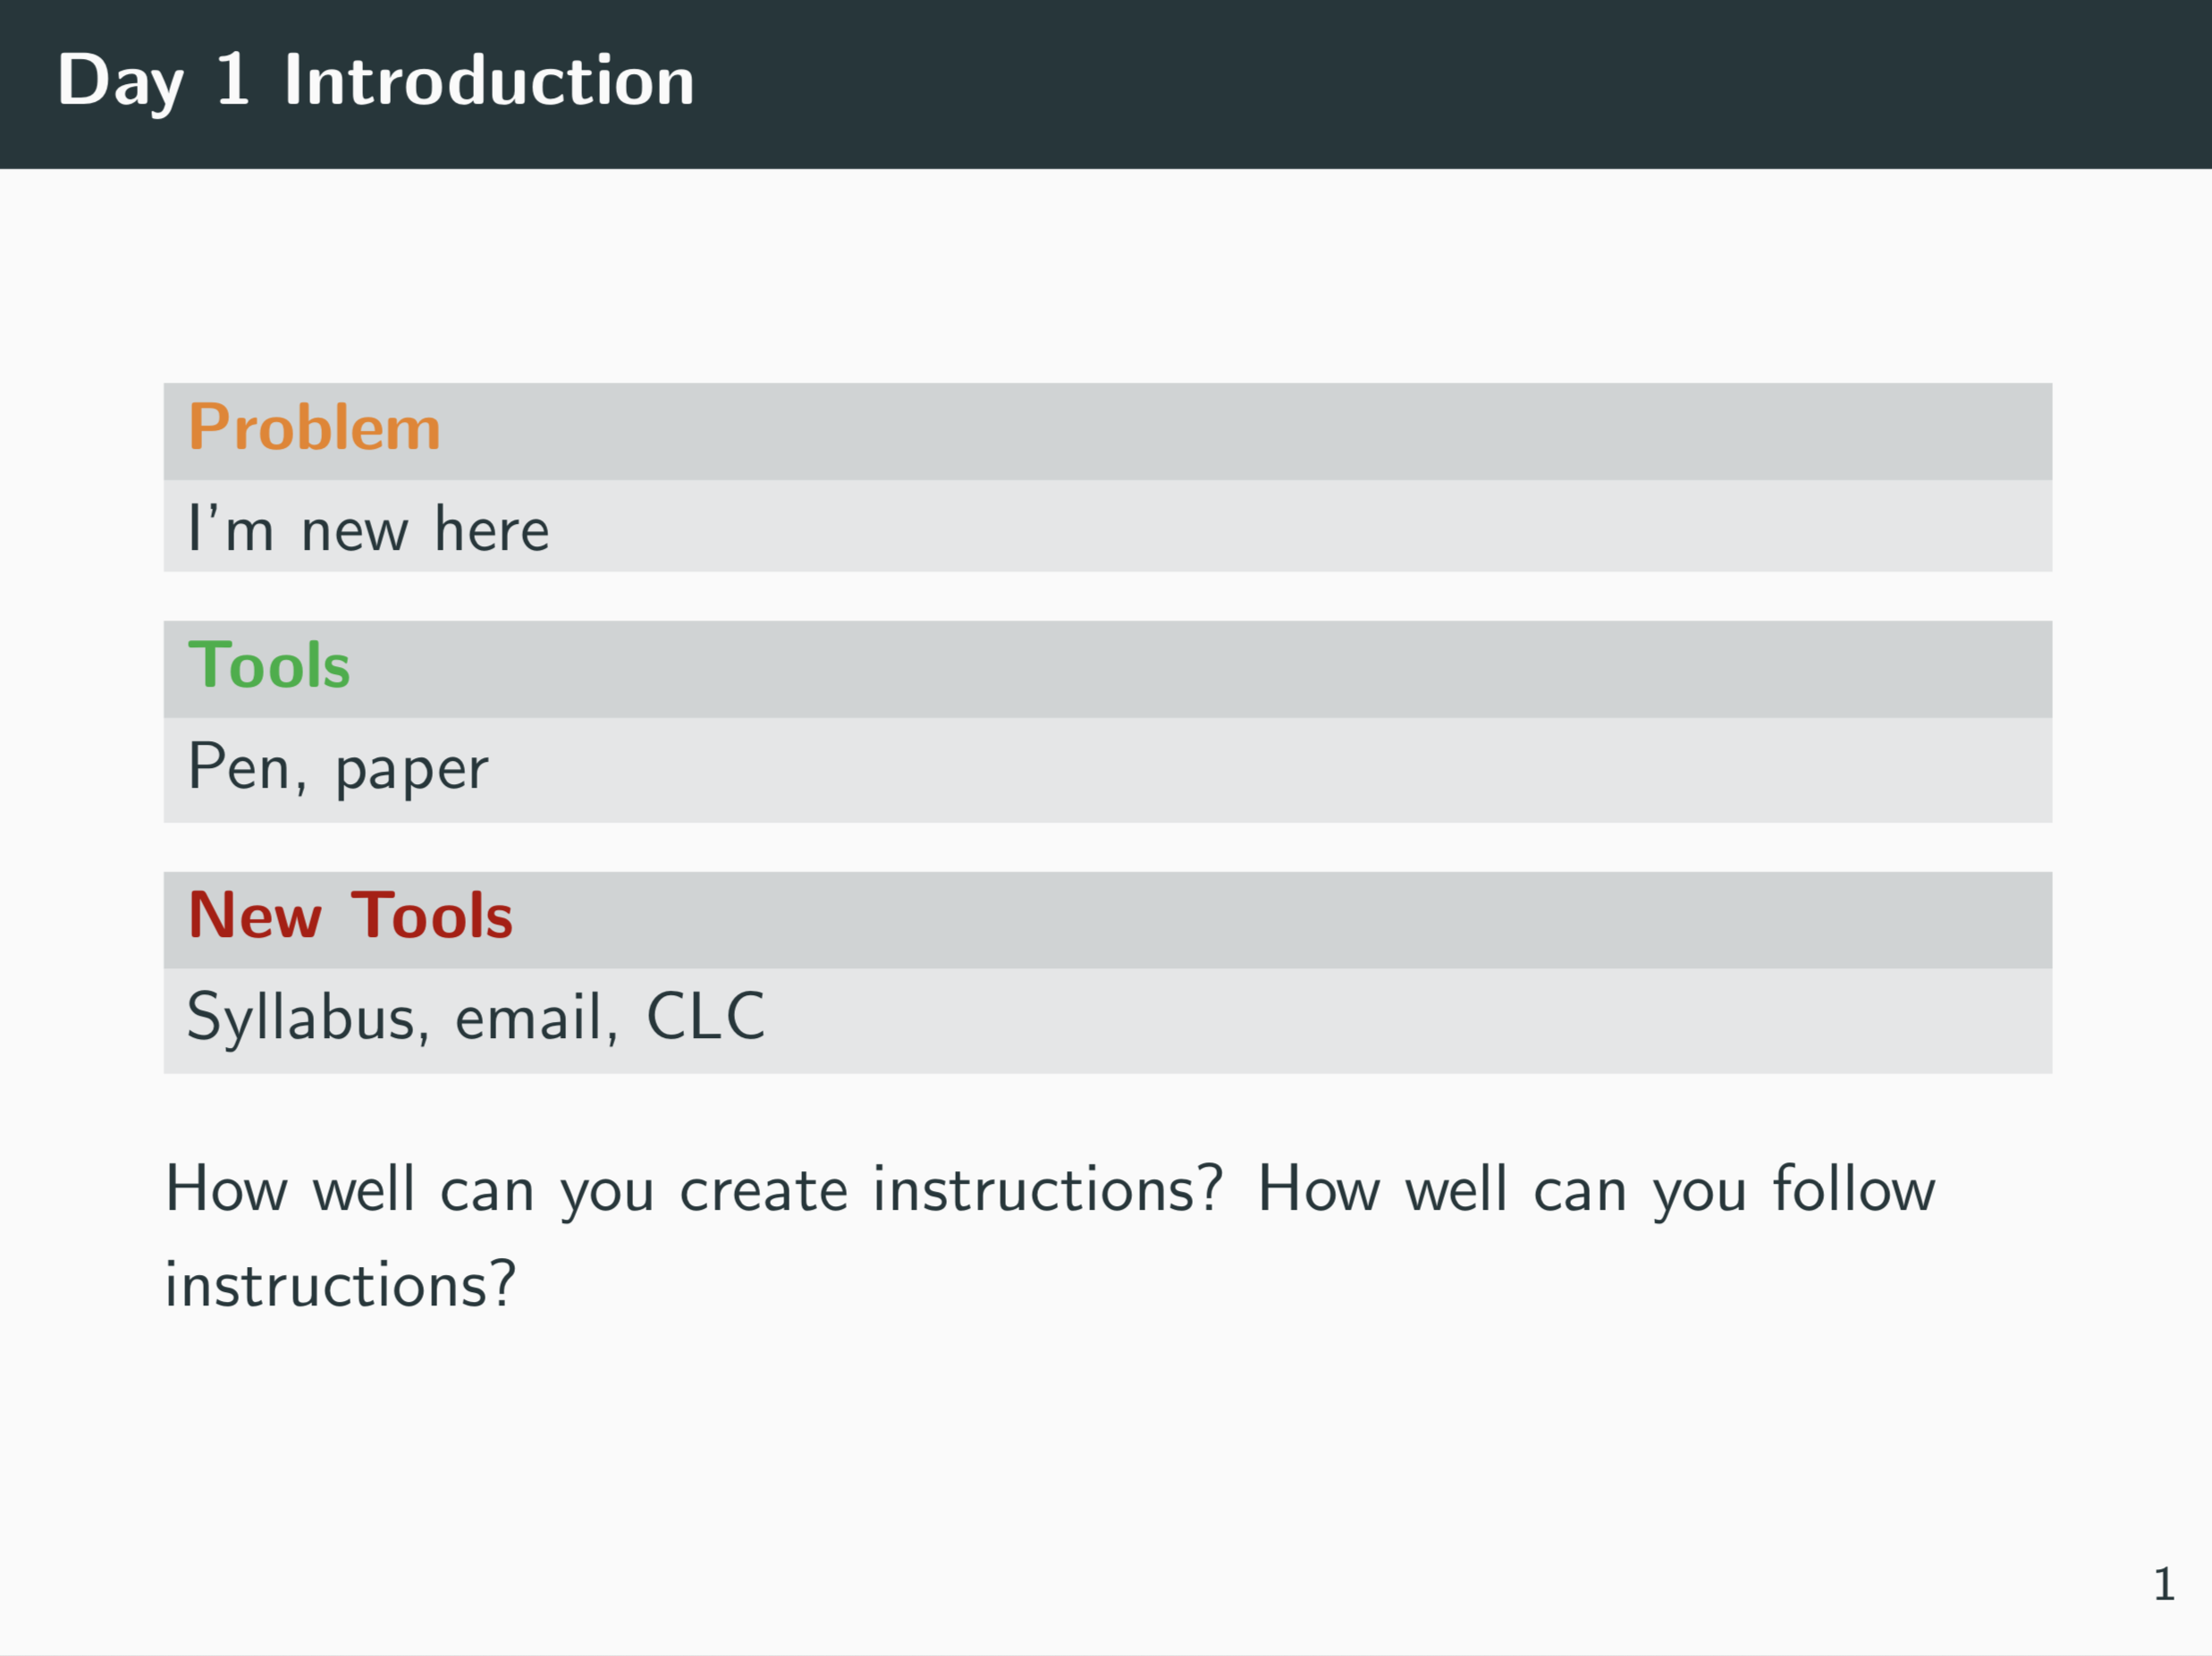
\includegraphics[scale=0.25]{day1slide}
\end{myfigure}

Understanding the day's problem, tools to be used, and new tools to be acquainted with, is a good way to get into the right mindset for the day's activities.

\section{Interview Questions}

It was once very popular for hiring officers to ask programmers to solve very difficult logic puzzles during job interviews.  These questions are no longer used so frequently, but they were popular because, it was thought, they allowed the interviewers to see how the interview subjects think about new problems.  As we work through the first part of this course, we will examine questions like this, to try to gain insight into how programmers think, and why it seems that programmers think about things in a different way than other people do.

The article that begins on Page \pageref{cnn} at the end of today's notes describes the situation well.

\section{Logo Exercise}

The best way to learn how to do anything is to do it.  Several times this semester, you will be engaging in a hands-on activity, meant to help you enhance a skill that you will be relying on throughout the rest of the course.  Today, you will learn just how difficult it can be to write directions and to follow them.

\section{Homework}

For homework, make sure you do the following things:
\begin{itemize}
\item Sign up for any web sites your professor asked you to sign up for, like the course management system, communications tools, etc.
\item Purchase access to the zyBooks textbook
\item Familiarize yourself with the location of the Computer Learning Center in B 225
\end{itemize}

\newpage
\label{cnn}
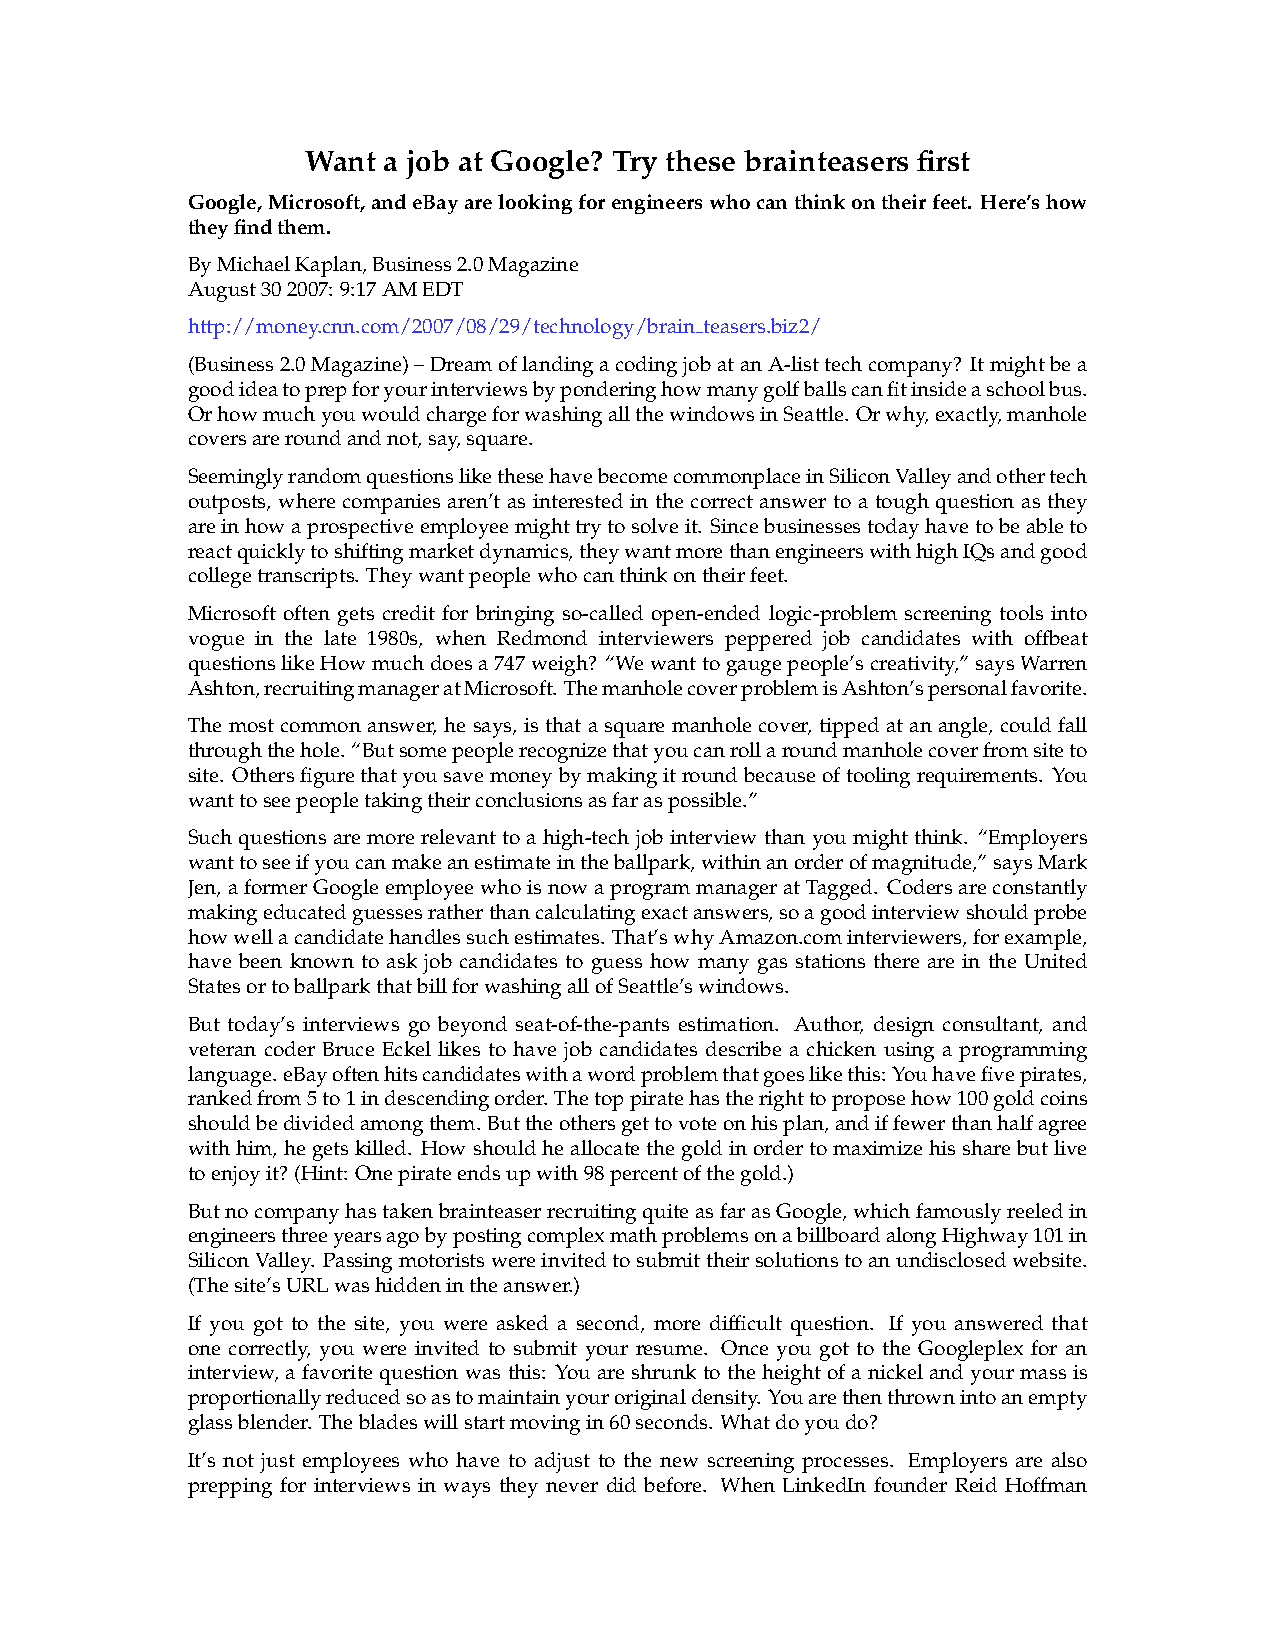
\includepdf[pages=-,pagecommand={\pagestyle{fancy}},noautoscale,scale=0.9]{day1-interview-article.pdf}

% !TEX root = CSC104LectureNotes.tex

\setcounter{chapter}{1}
\chapter{Talking Like a Programmer}
\label{day:vocabulary}

\topquote{It's all talk until the code runs.}{Ward Cunningham}

\minitoc

\section{Interview Question}

Your professor will give you a challenge regarding the crossing of a rope bridge.  Remember -- what's most important is that you make a guess, even if it isn't right.  A ``bad'' guess can help lead to the correct answer!

\section{Vocabulary}

Some people think, when they hear programmers talk, that they're speaking a foreign language.  Hopefully, today's lesson will help familiarize you with some of the jargon we use.  If you're going to do programming, it's important that you understand the spoken language that will be used, so that you can converse with the people you'll be working among.

\subsection{What Is a Computer Program?}

A \addindex{Program!Definition}{computer program} consists of a series of instructions that we humans write, using a vocabulary that the computer can understand.  When the computer \textit{executes}, or runs, our instructions, it will do so exactly as they are written, and so it's important that we write these instructions using the right language, in the right order, and without any ambiguity.

A person who is in the process of creating a program is said to be engaged in \addindex{Program!Programming}{computer programming}.  But programming isn't just the act of typing stuff on a keyboard; it also involves \textbf{testing} the program to see whether it works, and then \textbf{debugging}, or removing the problems we've programmed in.

\subsection{What Is an Algorithm?}

This leaves us with the question of what to type in.  How do we know which instructions to give to the computer?

The process of programming starts with designing an algorithm.  An \addindex{Algorithm}{algorithm} is a set of instructions that can be used repeatedly to solve a problem.  You probably have some algorithms you follow every day, like preparing breakfast or walking to class from the parking lot.  You could probably sit at home and describe to another student over the phone how to walk to the B building from where you normally park.  Some important characteristics of algorithms are that they're \textbf{repeatable} and \textbf{describable} to another person.

A programmer, then, describes an algorithm to a computer, by writing instructions in the computer's language.

\subsection{What's In a Computer?}

Most modern computers, whether on your desk or in your pocket, have these components:
\subsubsection{Central Processing Unit}
The \index{CPU|see {Central Processing Unit}}\addindex{Central Processing Unit}{central processing unit}, or \textbf{CPU}, is the part of the computer that performs all of the instructions we write.  It keeps track of what instruction needs to be performed next, and makes sure the right things show up on the screen and get stored in memory.  CPUs are frequently measured by how many billions of operations they can perform in a second, using the unit of measurement \textit{gigahertz} (GHz).

\subsubsection{Memory}
\label{sec:memory}
The computer's \addindex{Memory}{memory}, also called \textit{primary storage}, stores programs until they're ready to be run, and it also stores data and information that programs need while they run.  When you learn about \textit{variables} later, you will learn that they get stored here.

We measure the capacity of a computer's memory in \textit{gigabytes}, or how many billions of bytes it can store.  In a typical desktop computer, the memory used by programs (\textit{RAM}, or \textit{random access memory}) only works when there's a constant supply of electricity; if the computer loses power, the memory will be emptied.

\subsubsection{Drives, Disks, and Long-Term Storage}
There are many kinds of \textit{secondary storage} available for various kinds of computers.  They are frequently refered to as \addindex{Hard Drive}{hard drives} or \textit{disks}, although these terms don't apply to some of the newest choices.  Whether they use old-fashioned spinning platters or not, however, they are used to store lots of data for a long time, including when the computer is off.  Hard drives are used to store our programs when they're not in use, and our files, like term papers, saved game progress, and songs.

\subsubsection{Input and Output}
Keyboards, screens, mice, speakers, and similar devices allow us to \addindex{Input}{input} information into the computer, and allow the computer to \addindex{Output}{output} information back to us.  Computers can work just fine without these devices, but not in an interactive way.

\subsection{Kinds of Programming Errors}
\label{sec:kindsoferrors}

There are three broad categories of errors that can exist in a computer program.  The first is an error in the structure of our instructions, and the second is an error in the logic of our instructions.  (The third is an error in the execution of our instructions, but we'll talk about these kinds of errors later.)

A \addindex{Error!Syntax error}{syntax error} is an error that arises when we programmers type something that does not follow the structural rules of the programming language in which we're writing.  Consider a similar error in a natural language.  What's wrong with this English sentence?

\begin{myfigure}[label=fig:syntax-error-in-English]{A syntax error in English}
    \begin{tcolorbox}[floatplacement=h,width=\textwidth,colback=black!10]
        \centering
        \textbf{\textit{\large{This sentence no verb.}}}
    \end{tcolorbox}
\end{myfigure}

The problem there is that we broke the rules of English -- specifically, the rule that says a sentence has to have a verb.

Now consider this sentence:

\begin{myfigure}[label=fig:semantic-error-in-English]{A semantic error in English}
    \begin{tcolorbox}[floatplacement=h,width=\textwidth,colback=black!10]
        \centering
        \textbf{\textit{\large{My dog drove me to school today.}}}
    \end{tcolorbox}
\end{myfigure}

The structure of this sentence is valid.  A grammarian would have no problem with this sentence.  A logician, however, would bristle at this, because it doesn't make any sense.  The sentence in Figure \ref{fig:semantic-error-in-English} doesn't contain any syntax errors, but it does contain an error.  Specifically, this sentence has a \addindex{Error!Semantic error}{semantic error}, which is an error in the logic or meaning of a statement.

\subsection{How the Computer Reads Our Instructions}

Certainly we humans don't communicate with each other using computer programming languages, and so when we write programs, we're performing a sort of translation, or interpretation, of our algorithm into that language.  You may be surprised, however, to learn that even a programming language is not a computer's native language.  The only language the computer natively understands is numerical in nature -- instruction 1 might mean ``add these two numbers,'' and instruction 2 might mean ``compare these two numbers, and store the result over here.''  Therefore, we need a program to translate our computer programming language instructions -- which we call \addindex{Source code}{source code} -- into machine language instructions.  There are two ways this can happen.

Some languages utilize a program called a \addindex{Compiler}{compiler}, which examines all of our source code at once.  If all of the source code is free of syntax errors, the compiler will then translate the entire program to machine language code.  The code that comes from the compiler is saved on disk, and can be run multiple times without having to be compiled again.  Other languages' source code is fed into an \addindex{Interpreter}{interpreter}, which attempts to execute each instruction of a program separately.  An interpreter can run some of a program, even if there's a syntax error somewhere in the middle; however, once a syntax error is encountered, the interpreter will immediately exit.

The language we will be programming in this semester, called Python, is a compiled language, but the resulting code is not machine code.  Instead, the Python compiler creates something called \addindex{Bytecode}{bytecode}, which then must be run by an interpreter.

\section{Three Fundamental Components of a Program}
\label{sec:threekinds}

There are three basic kinds of instructions that we programmers can write when implementing our algorithms in computer code.

\subsection{Sequential Statements}

It's important for some instructions to take place in a certain order.  When you're making breakfast, you can't put your knife in the preserves jar if you haven't taken the lid off first.  \addindex{Statement!Sequential}{Sequential statements} must be typed in in the proper order when necessary.

\subsection{Selection Statements}

Did you plug in your mobile phone when you got to class today?  Why?  Is there a certain threshold of battery percentage at which you worry about it lasting through class?  We can write certain instructions for the computer to select what to do, based upon a condition.  \addindex{Statement!Selection}{Selection statements} (also known as \addindex{Statement!Conditional}{conditional statements}) allow us to allow the computer to make a decision.  We'll explore those more in a few weeks.  \index{Conditional statement|see {Statement}}

\subsection{Iteration Statements}

How was parking today?  Did you have to drive in circles around a section of the parking lot?  Any repeated action like that is called \textit{iteration} by programmers, and so an \index{Statement!Iteration|see {Loop}}\addindex{Statement!Loop}{iteration statement}, or \textit{loop}, is the kind of instruction we write when we want some task to happen over and over again.

\section{Programming Ethics}

From time to time in this course, we will discuss the responsibilities we programmers have to the people whose lives our work might affect.  The \href{https://www.acm.org/code-of-ethics}{Code of Ethics} published by the \href{https://www.acm.org/}{Association for Computing Machinery} is a resource that is widely accepted throughout the computing industry, and one to which all of us that teach Computer Science and Information Technology here at Nassau subscribe.

\subsection{General Principles}

The first part of the Code of Ethics lists a programmer's General Principles.  Our first principle is this:

\begin{tcolorbox}[width=\textwidth,colback=black!10]
Contribute to society and to human well-being, acknowledging that all people are stakeholders in computing.  [\href{https://www.acm.org/code-of-ethics#h-1.1-contribute-to-society-and-to-human-well-being,-acknowledging-that-all-people-are-stakeholders-in-computing.}{direct link}]
\end{tcolorbox}

This principle affirms our responsibility to use our talents for the benefit of society.  It is not only easy, but far too common, for people, organizations, and corporations to forget this principle and, either through mistakes or through overt acts, create software and computer systems that do not benefit society, and potentially even cause harm to people or computers.  Computers -- and, by extension, programmers -- have changed the world for the better, but we must always strive to maintain the trust that society has placed in us.

\section{Writing and Following Directions Exercise}

Your instructor is going to ask you and a partner to write some instructions, but with some restrictions.  Then we will see how you did.

\section{Homework for Day 3}

Ted and Ken, and their wives Allyson and Janie each have a favorite sport.  The sports they enjoy are running, swimming, biking, and golf.  Based upon these clues, determine whose favorite sport is which, and submit the answer for homework before Day 3 begins.  Your instructor will give you instructions for submitting your answer.
\begin{enumerate}
\item Ted hates golf.
\item Ken wouldn't run around the block if he didn't have to, and neither would his wife.
\item Each woman's sport is featured in a triathlon.
\item Allyson bought her husband a new bicycle for his birthday, to use in his favorite sport.
\end{enumerate}

% !TEX root = CSC104LectureNotes.tex

\newcommand{\mO}{\textbf{\textcolor{mLightGreen}{O}}}
\newcommand{\mX}{\textbf{\textcolor{mLightBrown}{X}}}

\setcounter{chapter}{2}
\chapter{Matrix Logic}

\topquote{Unfortunately, no one can be told what the Matrix is. You have to see it for yourself.}{Morpheus}

\minitoc

\section{What Is Matrix Logic?}

It can be hard to know how to solve a problem that has multiple elements and multiple possibilities.  Part of the transition into thinking like a programmer involves the ability to organize information and eliminate impossibilities in a systematic way.  A \addindex{Matrix}{matrix} helps us set up a one-to-one correspondence among the elements in a problem.

\section{Example Matrix Problem}

\textbf{The problem statement:} Three friends, Sarah, Natalie, and Charlotte, all had dates on Saturday night, with Nick, Matt, and Ben.  One couple went to the movies, one went to the park, and one went out to dinner.  Based on these text messages, see if you can determine who went out with whom, and where they went.

\begin{minipage}{\textwidth}
\textbf{The clues:}\\

\begin{tcolorbox}[width=\textwidth,colback=black!10]
5:45\\
Can't believe how cold it is and the grass is all wet, yuck. It's okay though, Matt gave me his coat, I think he really likes me.\\

8:34\\
Hey guys, hope you're having a better time than I am. Ben is such a bore, I don't think I'll be doing this again. xoxoxo love, Sarah oxoxox\\

9:24\\
Wow, this movie is fantastic and he's just as into it as I am. I don't think it'd ever be as fun with a geek like Matt (no offence). I don't ever want this to end. Good luck on your dates, love Natalie
\end{tcolorbox}
\end{minipage}

\textbf{The strategy:}  Did Sarah go out with Ben?  Did Natalie go to the park?  We need a system of solving this problem that helps us eliminate the combinations that couldn't have happened, so that we leave only the one solution that makes sense.

For a problem like this, the best strategy is to create a \textbf{matrix} like this:

\begin{myfigure}[label=fig:datesmatrix]{Dates Problem Matrix}
    \begin{tcolorbox}[width=\textwidth,colback=black!10]
        \begin{center}
            \begin{tabular}{r|c|c|c||c|c|c|}
                & Nick & Matt & Ben & Movies & Park & Dinner\\
                \hline\hline
                Sarah & & & & & & \\
                \hline
                Natalie & & & & & &\\
                \hline
                Charlotte & & & & & & \\
                \hline\hline
                Movies & & & \\
                \cline{1-4}
                Park & & & \\
                \cline{1-4}
                Dinner & & &\\
                \cline{1-4}
            \end{tabular}
        \end{center}
    \end{tcolorbox}
\end{myfigure}

Some of the clues in a problem like this help us match two pieces of information.  We will place a capital letter \mO{} where we have a match.  Read the first text message again.  We don't know who sent it, but we know she's in the park with Matt, so we can update the matrix like this:

\begin{tcolorbox}[width=\textwidth,colback=black!10]
    \begin{center}
        \begin{tabular}{r|c|c|c||c|c|c|}
            & Nick & Matt & Ben & Movies & Park & Dinner\\
            \hline\hline
            Sarah & & & & & & \\
            \hline
            Natalie & & & & & &\\
            \hline
            Charlotte & & & & & & \\
            \hline\hline
            Movies & & & \\
            \cline{1-4}
            Park & & \mO{} & \\
            \cline{1-4}
            Dinner & & &\\
            \cline{1-4}
        \end{tabular}
    \end{center}
\end{tcolorbox}

Once we've placed the O, it becomes clear that neither Nick nor Ben is at the park, and that Matt is neither at the movies nor at dinner.  We can mark these impossibilities with an \mX{}, like this:

\begin{tcolorbox}[width=\textwidth,colback=black!10]
    \begin{center}
        \begin{tabular}{r|c|c|c||c|c|c|}
            & Nick & Matt & Ben & Movies & Park & Dinner\\
            \hline\hline
            Sarah & & & & & & \\
            \hline
            Natalie & & & & & &\\
            \hline
            Charlotte & & & & & & \\
            \hline\hline
            Movies & & \mX{} & \\
            \cline{1-4}
            Park & \mX{} & \mO{} & \mX{} \\
            \cline{1-4}
            Dinner & & \mX{} &\\
            \cline{1-4}
        \end{tabular}
    \end{center}
\end{tcolorbox}

The second text message tells us that Sarah is out with Ben.  This means that Sarah is not with Nick or Matt, and that Ben is not with Natalie or Charlotte:

\begin{tcolorbox}[width=\textwidth,colback=black!10]
    \begin{center}
        \begin{tabular}{r|c|c|c||c|c|c|}
            & Nick & Matt & Ben & Movies & Park & Dinner\\
            \hline\hline
            Sarah & \mX{} & \mX{} & \mO{} & & & \\
            \hline
            Natalie & & & \mX{} & & &\\
            \hline
            Charlotte & & & \mX{} & & & \\
            \hline\hline
            Movies & & \mX{} & \\
            \cline{1-4}
            Park & \mX{} & \mO{} & \mX{} \\
            \cline{1-4}
            Dinner & & \mX{} &\\
            \cline{1-4}
        \end{tabular}
    \end{center}
\end{tcolorbox}

But there's more information to glean from this clue.  Since we already know that Ben is not at the park, then neither is Sarah, and so we can eliminate that possibility as well:

\begin{tcolorbox}[width=\textwidth,colback=black!10]
    \begin{center}
        \begin{tabular}{r|c|c|c||c|c|c|}
            & Nick & Matt & Ben & Movies & Park & Dinner\\
            \hline\hline
            Sarah & \mX{} & \mX{} & \mO{} & & \mX{} & \\
            \hline
            Natalie & & & \mX{} & & &\\
            \hline
            Charlotte & & & \mX{} & & & \\
            \hline\hline
            Movies & & \mX{} & \\
            \cline{1-4}
            Park & \mX{} & \mO{} & \mX{} \\
            \cline{1-4}
            Dinner & & \mX{} &\\
            \cline{1-4}
        \end{tabular}
    \end{center}
\end{tcolorbox}

From the third text message, we learn that Natalie is at the movies.  Since Ben is out with Sarah, and Matt is at the park, Natalie must be out with Nick.

\begin{tcolorbox}[width=\textwidth,colback=black!10]
    \begin{center}
        \begin{tabular}{r|c|c|c||c|c|c|}
            & Nick & Matt & Ben & Movies & Park & Dinner\\
            \hline\hline
            Sarah & \mX{} & \mX{} & \mO{} & & \mX{} & \\
            \hline
            Natalie & \mO{} & \mX{} & \mX{} & \mO{} & \mX{} & \mX{} \\
            \hline
            Charlotte & \mX{} & & \mX{} & & & \\
            \hline\hline
            Movies & \mO{} & \mX{} & \\
            \cline{1-4}
            Park & \mX{} & \mO{} & \mX{} \\
            \cline{1-4}
            Dinner & & \mX{} &\\
            \cline{1-4}
        \end{tabular}
    \end{center}
\end{tcolorbox}

We are just about done with this problem at this point.  Notice that in the lower left, once the \mX{}'s are filled at Nick/Dinner and at Ben/Movies, it's clear that Ben is at Dinner, which means that Sarah is at dinner.  Similarly, with two \mX{}'s under Park in the top right, it must be Charlotte at the park, which means that that first text message, about Matt, was from her.

\begin{tcolorbox}[width=\textwidth,colback=black!10]
    \begin{center}
        \begin{tabular}{r|c|c|c||c|c|c|}
            & Nick & Matt & Ben & Movies & Park & Dinner\\
            \hline\hline
            Sarah & \mX{} & \mX{} & \mO{} & \mX{} & \mX{} & \mO{} \\
            \hline
            Natalie & \mO{} & \mX{} & \mX{} & \mO{} & \mX{} & \mX{} \\
            \hline
            Charlotte & \mX{} & \mO{} & \mX{} & \mX{} & \mO{} & \mX{} \\
            \hline\hline
            Movies & \mO{} & \mX{} & \mX{} \\
            \cline{1-4}
            Park & \mX{} & \mO{} & \mX{} \\
            \cline{1-4}
            Dinner & \mX{} & \mX{} & \mO{} \\
            \cline{1-4}
        \end{tabular}
    \end{center}
\end{tcolorbox}

And so: Sarah and Ben are at dinner, Natalie and Nick are at the movies, and Charlotte and Matt are at the park.

\section{Matrix Logic Exercises and Homework}

You will have the opportunity to solve a couple of problems like this in class.  Answers to the last one should be submitted for homework.
% !TEX root = CSC104LectureNotes.tex

\setcounter{chapter}{3}
\chapter{Systematic Lists}

\topquote{It's not that I'm so smart, it's just that I stay with problems longer.}{Albert Einstein}

\minitoc

\section{Interview Question}

Day \thechapter{} starts with an interview question about the competitors in a tournament.  See if you can answer the question without help.  If not, see if a nearby classmate can give you a hint.

\section{Systematic Lists}

A \addindex{Systematic List}{systematic list} is a list of related items that are listed in a predetermined order.  The ability to create such a list is a skill that programmers use in solving a certain kind of problem.

\subsection{Why Use Systematic Lists?}

Creating a systematic list is a great way to explore \textit{combinations} of items or values.  Here's an example:  Suppose that Allison, Becky, and Charlotte are running a race.  What are all the race results that can happen?  It's possible for Becky to win, followed by Charlotte and then Allison, but it's also possible for Allison to win, followed by Charlotte and then Becky.

It seems like human nature for us to discuss these possible results in this way, by discussing each result as we think of it.  However, there are two potential problems in this scenario:
\bi
    \item There is no way to be sure that we haven't skipped any results
    \item There is no way to know that we completed the task
\ei

Using a systematic list helps solve both of those problems.

\subsection{How Do We Create a Systematic List?}

The best way to avoid these problems is to attack each situation the same way.  We will develop an \textit{algorithm}, and follow it.  A successful algorithm will not only work every time, but finish as soon as it has to.

An \addindex{Algorithm}{algorithm} is, according to Merriam-Webster, ``a step-by-step procedure for solving a problem or accomplishing some end.''  A good algorithm should be \textit{describable}, \textit{repeatable}, and \textit{verifiable} -- that is, we should be able to talk about it, use it, and know it works.

The most successful algorithm for creating a systematic list relies heavily upon the \textit{order} of the items to be listed.  Notice, in our previous example, that the race runners have a natural ordering criteria -- we can alphabetize their names.  A statement like ``Becky's name comes before Charlotte's'' makes sense to us.  We will use this feature of people's names to our advantage.

Our systematic list algorithm involves repeating this step over and over:
\bi
    \item Add the smallest unused value in the left-most available position
    \item Only use the next value when all combinations utilizing the present value have been enumerated
\ei

\subsection{Creating a Systematic List}

We will fill in this table with as many rows as we need:

\begin{center}
    \begin{tabulary}{\textwidth}{CCC}
        First Place & Second Place & Third Place\\
        \hline
        \textit{result} & \textit{result} & \textit{result}
    \end{tabulary}
\end{center}

Using our race running example, the ``first'' name we have available is Allison, and so we will start by enumerating all of the race results in which she is the winner.  Let's place Allison in the left-most position.

\begin{center}
    \begin{tabulary}{\textwidth}{CCC}
        First Place & Second Place & Third Place\\
        \hline
        Allison & \textit{result} & \textit{result}
    \end{tabulary}
\end{center}

Once we've done that, as the algorithm says, we will add the smallest unused value in the left-most available position.  The ``smallest'' name we haven't used yet is Becky's, and the left-most available position is next to Allison.

\begin{center}
    \begin{tabulary}{\textwidth}{CCC}
        First Place & Second Place & Third Place\\
        \hline
        Allison & Becky & \textit{result}
    \end{tabulary}
\end{center}

There is one more spot in this row to fill, and one more name -- the ``largest'' or latest alphabetically -- to add.

\begin{center}
    \begin{tabulary}{\textwidth}{CCC}
        First Place & Second Place & Third Place\\
        \hline
        Allison & Becky & Charlotte
    \end{tabulary}
\end{center}

Because there are no other names to replace Charlotte's with, we will consider ourselves done with all of the combinations that start with \textit{Allison and Becky}.

Note, however, that there are more possible results that start with Allison.  Let's backtrack to that scenario:

\begin{center}
    \begin{tabulary}{\textwidth}{CCC}
        First Place & Second Place & Third Place\\
        \hline
        Allison & Becky & Charlotte\\
        Allison & \textit{result} & \textit{result}
    \end{tabulary}
\end{center}

Remember what our algorithm tells us to do:  \textit{Add the smallest unused value in the left-most available position}.  The smallest name we haven't used for second place yet is Charlotte, so let's add her:

\begin{center}
    \begin{tabulary}{\textwidth}{CCC}
        First Place & Second Place & Third Place\\
        \hline
        Allison & Becky & Charlotte\\
        Allison & Charlotte & \textit{result}
    \end{tabulary}
\end{center}

In this row, we have used Allison's name and we have used Charlotte's name, but we have not used Becky's name.  The algorithm tells us to \textit{Add the smallest unused value in the left-most available position}.  That means add Becky to the third column:

\begin{center}
    \begin{tabulary}{\textwidth}{CCC}
        First Place & Second Place & Third Place\\
        \hline
        Allison & Becky & Charlotte\\
        Allison & Charlotte & Becky\\
    \end{tabulary}
\end{center}

Since we've now used every runner's name in this row, we can conclude that there are no more combinations that start with \textit{Allison and Charlotte}.

Let's backtrack once again:

\begin{center}
    \begin{tabulary}{\textwidth}{CCC}
        First Place & Second Place & Third Place\\
        \hline
        Allison & Becky & Charlotte\\
        Allison & Charlotte & Becky\\
        Allison & \textit{result} & \textit{result}
    \end{tabulary}
\end{center}

Are there any more combinations that start with just \textit{Allison}?  In other words, if Allison wins the race, are there any other orders in which the runners can finish?

The algorithm says \textit{Add the smallest unused value in the left-most available position}.  But here in Column 2, there are no more unused values.  The next part of the algorithm says  \textit{Only use the next value when all combinations utilizing the present value have been enumerated}.  Since we have now enumerated all of the conditions utilizing the present value -- that is, we've listed all the results possible when Allison wins -- we are now free to use the next value.

\begin{center}
    \begin{tabulary}{\textwidth}{CCC}
        First Place & Second Place & Third Place\\
        \hline
        Allison & Becky & Charlotte\\
        Allison & Charlotte & Becky\\
        \sout{Allison} & \sout{\textit{result}} & \sout{\textit{result}}
    \end{tabulary}
\end{center}

In this case, the next value is the next smallest value in Column 1, meaning it's time to see what can happen if Becky wins the race.

\begin{center}
    \begin{tabulary}{\textwidth}{CCC}
        First Place & Second Place & Third Place\\
        \hline
        Allison & Becky & Charlotte\\
        Allison & Charlotte & Becky\\
        Becky & \textit{result} & \textit{result}
    \end{tabulary}
\end{center}

At this step, we ask once again what the smallest remaining value is.  We haven't used Allison's name in this row yet, so we put her name into Column 2 now.

\begin{center}
    \begin{tabulary}{\textwidth}{CCC}
        First Place & Second Place & Third Place\\
        \hline
        Allison & Becky & Charlotte\\
        Allison & Charlotte & Becky\\
        Becky & Allison & \textit{result}
    \end{tabulary}
\end{center}

That leaves Charlotte to finish third:

\begin{center}
    \begin{tabulary}{\textwidth}{CCC}
        First Place & Second Place & Third Place\\
        \hline
        Allison & Becky & Charlotte\\
        Allison & Charlotte & Becky\\
        Becky & Allison & Charlotte\\
    \end{tabulary}
\end{center}

As before, there is another name available to put right after Becky's:

\begin{center}
    \begin{tabulary}{\textwidth}{CCC}
        First Place & Second Place & Third Place\\
        \hline
        Allison & Becky & Charlotte\\
        Allison & Charlotte & Becky\\
        Becky & Allison & Charlotte\\
        Becky & Charlotte & Allison\\
    \end{tabulary}
\end{center}

There is only one winner left to explore, and we complete the systematic list by completing the algorithm:

\begin{center}
    \begin{tabulary}{\textwidth}{CCC}
        First Place & Second Place & Third Place\\
        \hline
        Allison & Becky & Charlotte\\
        Allison & Charlotte & Becky\\
        Becky & Allison & Charlotte\\
        Becky & Charlotte & Allison\\
        Charlotte & Allison & Becky\\
        Charlotte & Becky & Allison\\
    \end{tabulary}
\end{center}

\section{Characteristics of a Systematic List}

When you are asked to produce a systematic list of all the outcomes of this race, it is not enough to just list all of the outcomes; they must be listed in the proper order.  You must create a systematic list, not just a list.

The system in this list lies in the ordering.  First, notice that the values in the first column never decrease.  All of the outcomes in which Allison wins are listed before any of the others, and all of the outcomes in which Becky wins are listed before any in which Charlotte wins.

Then, when you consider all of the outcomes that have the same first-column value, notice that the second-column values are also written in non-decreasing order -- Becky then Charlotte, Allison then Charlotte, and Allison then Becky.

\section{Creating Systematic Lists}

Follow your instructor's lead in creating some systematic lists in class.
% !TEX root = CSC104LectureNotes.tex

\chapter{Binary Numbers}

\topquote{There are 10 kinds of people in this world -- those who understand binary numbers, and those who don't.}{A progammer's t-shirt}

\minitoc

\section{Review Exercise}
\label{sec:syslistreview}

Your instructor will ask you to create a systematic list to help you review what you learned in Day 4, and also to help introduce today's topic.

\section{What Is a Number System?}

A \textbf{number system} is a series of symbols that we use to represent numeric values.  We are used to using \addindex{Decimal numbers}{decimal numbers} in our daily lives.  This number system, as indicated by the Greek root \textit{deci}, meaning ``ten,'' has ten digits -- namely, 0 through 9.  With those ten digits, we can describe any number we're thinking of.

If we create a systematic list of two-digit combinations of the digits 0 through 9, what emerges is a list of numbers between 0 and 99, in numeric order:  00, 01, 02, $\ldots$, 09, 10, 11, 12, $\ldots$, 39, 40, 41, $\ldots$, 98, 99.

Now consider a longer number, like 3284.  Each of those digits has a \textit{place name} -- there's a ones place, and a tens place, and so forth.  Why are those the names of the places?  Because that number is the same as \textit{three thousands, two hundreds, eight tens, and four ones}.

But why?  Well, it is no coincidence that each of those place names is equal to a power of ten.  Notice:

\[
\begin{array}{rclclclcl}
    3284 & = & 3 \cdot 1000 & + & 2 \cdot 100 & + & 8 \cdot 10 & + & 4 \cdot 1\\
         & = & 3 \cdot 10^3 & + & 2 \cdot 10^2 & + & 8 \cdot 10^1 & + & 4 \cdot 10^0\\
\end{array}
\]

Notice that for each of those exponents, the base is ten -- hence, this number was written in \textit{base ten}.

\section{Binary Numbers}
    
It might surprise you to learn that programmers sometimes use a number system other than base ten when discussing what happens inside a computer.

At its most basic hardware level, all a computer can recognize is things like whether a voltage is above or below a certain threshold, or whether a switch is open or closed, or whether a chunk of metal is aligned magnetically north or south.  All of these situations -- high or low, open or closed, yes or no -- represent \textbf{binary} states.  (The Greek root \textit{bi} shows up in other words you recognize, like \textit{bicycle} and \textit{bilingual}, and it means ``two.'')

Due to this tendency of computer components to exist in one of two binary states, we use \addindex{Binary numbers}{binary numbers} to represent these states.

Just like decimal numbers, each digit in binary numbers represents a base and an exponent.  With these numbers, however, the base for each exponent is two -- hence, \textit{base two} numbers.  The rightmost column in a binary number represents the $2^0$ place, or the \textit{ones place}; the middle column is the $2^1$ or \textit{twos place}; and the left column is the $2^2$, or \textit{fours place}.  Therefore, starting from the top, those three-binary-digit sequences represent the decimal numbers 0 through 7.  By the time you are done with the activities in Day \thechapter, you should be able to convert any decimal number within a certain range to binary, and vice versa.
% !TEX root = CSC104LectureNotes.tex

\setcounter{chapter}{5}
\chapter{Introduction to Conditionals}
\label{day:conditionals1}

\topquote{If you don't know anything about computers, just remember that they are machines that do exactly what you tell them but often surprise you in the result. }{Richard Dawkins}

\minitoc

\section{Decisions}

Life is full of decisions.  Some decisions, like \textit{should I change my major to Computer Science?}{} are very important, whereas others, like \textit{should we go to Wendy's or Taco Bell for lunch?}{} only seem important at the time.

The earliest computer programmers faced decisions as well.  Should this employee be paid a straight wage, or overtime?  Is this user's input valid?  Computers were designed to be good at handling decision making like this.

\section{Conditions and Boolean Values}

A \addindex{Condition}{condition} is something that is either true or false.  \textit{It is cold out} is a condition -- you can determine for yourself as you read this whether that statement is true or false right now.  In a few hours, or a few months, it is possible for this condition to have the opposite value.

As we start to discuss how to write computer programs, the conditions with which we will deal most frequently will involve \textit{comparisons}.  We will learn how to ask questions like ``Are you older than 21 years old?,'' and how to perform different tasks based on the possible outcomes.

English mathematician George Boole is usually credited with first formalizing the way we write about conditions and comparisons.  His system came to be known as \textit{Boolean logic}.  Similariy, the values \texttt{False} and \texttt{True} -- the only two values a condition in Boolean logic can have -- are referred to as \textit{Boolean values}.  \texttt{False} and \texttt{True} are the only two Boolean values.

Today's lesson will focus on the use of \addindex{Operators!Relational operators}{relational operators}, which help us create a condition that examines the relationship between two values.  These operators help us talk about ideas like ``this number is less than that number,'' or ``this number is greater than or equal to that number.''

In math class, you may have encountered statements like $x \ge y$, which means ``$x$ is greater than or equal to $y$.''  This is difficult to type, however, because there is no $\ge$ key on your keyboard.  Every programming language defines a set of operators that programmers must type to express these otherwise-untypeable ideas.  Table \ref{tab:relational} presents the relational operators you will need to know when we start programming in Python.

\begin{mytable}[label=tab:relational]{Relational Operators in Python}
        \begin{tabulary}{\linewidth}{ccc}
            Mathematical Symbol & Meaning & Python Code\\
            \hline
            $<$ & Less Than & \texttt{<}\\
            $\le$ & Less Than or Equal & \texttt{<=}\\
            $>$ & Greater Than & \texttt{>}\\
            $\ge$ & Greater Than or Equal & \texttt{>=}\\
            $=$ & Equal & \texttt{==}\\
            $\neq$ & Not Equal & \texttt{!=}\\
            \hline
        \end{tabulary}
\end{mytable}

As you work through the examples today and over the next few days of class, make sure you use the Python operators, not the mathematical operators.  You will use these operators today while you learn the format for a \addindex{Statement!Conditional}{conditional statement} and how to create your own.  In later lessons you will write increasingly complex conditional statements.

While writing and testing conditional statements, make sure you pay attention to the idea of a \textbf{\textit{possible value}} to be evaluated in a condition (this is the number you will compare to the \textit{present state} of something), and make sure you understand how to determine the possible \textbf{\textit{outcomes}} of a conditional statement.
% !TEX root = CSC104LectureNotes.tex

\setcounter{chapter}{6}
\chapter{Nested Conditionals and Complex Conditonals}

\topquote{The most important property of a program is whether it accomplishes the intention of its user.}{C.\ A.\ R.\ Hoare}

\minitoc

\section{Nested Conditionals}

We learned in Day \ref{day:conditionals1} that a condition can only have one of two values, \texttt{True} or \texttt{False}, and therefore a \textit{conditional statement} can only have two possible \textit{outcomes}.  These ideas make conditional statements very useful for certain problems in life, but there are situations that need more complex tools than these.

Consider, for example, running into an old middle school classmate in town.  You remember each other, and realize quickly that you haven't seen each other since middle school.  Your friend says, ``So what happened to you?  Did you go to Kellenberg or something?''  If you didn't, then you might be surprised if your friend follows up with ``Oh, I guess you went to St.\ Anthony's.''  Even if you \textit{did} go to to St.\ Anthony's, that statement illustrates quite a gap in your friend's logical reasoning skills.

The problem is that the conditional statement that's implied here has more \textit{outcomes} than your friend has considered.  Her thinking appears to work like Figure \ref{fig:hs1}.

\begin{myfigure}[label=fig:hs1]{Flawed Thinking About High School}
    \begin{minipage}{0.925\linewidth}
        \centering
        \begin{tikzpicture}
            \centering
            \node[decision,text width=6em](hs) {Did you go to Kellenberg?};

            \node[block,below left = of hs](yes) {You went to Kellenberg};
            \node[block,below right = of hs](no) {You went to St.\ Anthony's};

            \path[line] (hs) -| (yes) node[near start, above=0.5em] {Yes};
            \path[line] (hs) -| (no) node[near start, above=0.5em] {No};
        \end{tikzpicture}
    \end{minipage}
\end{myfigure}

Of course, your friend should be thinking like Figure \ref{fig:hs2} instead.

\begin{center}
    \begin{myfigure}[label=fig:hs2]{Less Flawed Thinking About High School}
        \begin{tikzpicture}
            \centering
            \node[decision,text width=6em](hs) {Did you go to Kellenberg?};

            \node[block,below = 3em of hs](sta) {You went to St.\ Anthony's};
            \node[block,left = of sta](k) {You went to Kellenberg};
            \node[nebula,right = of sta](others) {You went somewhere else};

            \path[line] (hs) -| node[near start,above=0.5em] {Yes} (k);
            \path[line] (hs) -- (sta) node[near end,above right=0.5em] {No};
            \path[line] (hs) -| node[near start,above=0.5em] {\textcolor{red}{Also no, but in red}} (others);
        \end{tikzpicture}
    \end{myfigure}
\end{center}

This is problematic, too.  We haven't learned about a conditional with three or more outcomes.  There's a simple reason for that -- \textit{there aren't any}.  The whole idea of a condition is that it's either False or True.  There is no third Boolean value.

Since a single conditional statement can only have two outcomes, what's needed in a scenario like this is multiple conditional statements.  Let's consider another example: you and your classmates all fall into one of three categories: you're either a Computer Science major, an Information Technology major, or your majoring in something else.  If you ask one of your classmates ``Are you a Computer Science major?'', the two outcomes are:

\begin{itemize}
    \item \textbf{Yes:} Now you know the student's major
    \item \textbf{No:} You don't know what the student's major is, but you know it's either IT or something else
\end{itemize}

If your classmate's answer is ``Yes'', you're done with the conversation.  If, however, the answer is ``No'', then there are still two possible outcomes.  Fortunately, you know how to deal with two possible outcomes -- use a conditional statement!  Consider Figure \ref{fig:csmajor}:

\begin{center}
    \begin{myfigure}[label=fig:csmajor]{Determining a Student's Major With a Nested Conditional}
        \begin{tikzpicture}[node distance=0.5cm]
            \tikzstyle{background}=[rectangle, %dashed,
                draw=mLightBrown, fill=mDarkGreen,
                inner sep=0.3cm, rounded corners=5mm]
            \node[decision](csq) {Are you a CS major?};

            \node[block, below left = of csq] (cs) {You're a CS major};
            \node[dummy,below right = of csq](dummy){~};

            \node[decision, below = 1cm of dummy](itq) {Are you an IT major?};

            \node[block, below left = of itq](it) {You're an IT major};
            \node[block, below right = of itq](other) {Your major is something else};

            \path[line] (csq) -| node[near start,above=0.5em] {Yes} (cs);
            \path[line] (csq) -| node[near start, above=0.5em] {No} (itq);

            \path[line,mLightBrown,thick] (itq) -| node[near start,above=0.5em] {Yes} (it);
            \path[line,mLightBrown,thick] (itq) -| node[near start,above=0.5em] {No} (other);

            \begin{pgfonlayer}{background}
                \node [background,
                       fit=(itq) (it) (other)] {};
              \end{pgfonlayer}
        \end{tikzpicture}
    \end{myfigure}
\end{center}

The shaded box contains a \addindex{Statement!Conditional!Nested}{nested conditional}.  After asking the first question (is major equal to Computer Science), if the answer is no, you have to \textit{ask another question}.  In this scenario, where there are three outcomes, two questions are necessary to arrive at the right answer.  In general, you must ask $n-1$ questions when choosing from among $n$ outcomes.

Creating a \addindex{Decision tree}{decision tree} like this is a good way to start thinking about how to write a nested conditional statement.  Once the picture is done, you can just read your decision tree from top to bottom and translate it into code.  Note that Python accomplishes nesting conditionals like this with the \mintinline{python}{elif} clause.  We will be using \mintinline{python}{elif} in our examples today and in the next few classes.

Here's the conditional statement that matches this decision tree:

\begin{verbatim}
if major = CS:
    "You're a CS major"
elif major = IT:
    "You're an IT major"
else:
    "Your major is something else"
\end{verbatim}

\section{Complex Conditionals}

What will make you attend the next class meeting of CSC 104?  A couple of things have to be true: it has to be a \textit{day} on which the class meets, and it has to be a \textit{time} when the class is meeting.  If your class meets at 2:00 pm on Wednesday, then showing up at 9:30 on Wednesday isn't going to help you, and neither is arriving at 2:00 pm on Thursday.

Then again, sometimes only one thing must be true for an outcome to occur.  If you're thirsty, you will drink some water.  But you will also drink some water if you have to take a pill.  You don't wait until both conditions are true before taking a drink of water; just one condition being true is sufficient.

Both of these scenarios can be handled using a \addindex{Statement!Conditional!Complex}{complex conditional}.  These scenarios are similar to those from Day \ref{day:conditionals1} in that there are only one or two outcomes (and therefore no nesting is necessary), but they're different in that many individual conditions go into determining which outcome happens.  In these cases, we must rely on a new set of operators.

\subsection{Boolean Operators}

\addindex{Operators!Boolean operators}{Boolean operators} allow us to create a condition by combining other conditions together.  You know these operators as ``and'', ``or'', and ``not''.  You may also recognize them in symbol form from your high school symbolic logic section: $\land$, $\lor$, and $\lnot$.

Recall your high school truth tables, as in Table \ref{tab:truthtables}:
\begin{center}
    \begin{mytable}[label=tab:truthtables]{And, Or, and Not Truth Tables}
        \begin{tabulary}{5in}{CCC|C|C}
            $x$ & $y$ & $x \land y$ & $x \lor y$ & $\lnot x$\\
            \hline
            F & F & F & F & T\\
            F & T & F & T & T\\
            T & F & F & T & F\\
            T & T & T & T & F\\
            \hline
        \end{tabulary}
    \end{mytable}
\end{center}

$x \land y$ (``x and y'') is only true if both $x$ and $y$ are true; otherwise it's false.  $x \lor y$ (``x or y'') is only false if both $x$ and $y$ are false; otherwise it's true.

Thankfully, Python does not require us to type the $\land$, $\lor$, and $\lnot$ symbols (which is good, because they aren't on the keyboard); we can just use \mintinline{python}{and}, \mintinline{python}{or}, and \mintinline{python}{not}.

With those operators, we can say things like ``If it's Wednesday \mintinline{python}{and} it's 2:00 pm, then I will go to CSC 104'', or ``If I'm thirsty \mintinline{python}{or} I need to take a pill, then I will drink water.''

\section{Writing Conditional Statements}

When you are asked to create a conditional statement from scratch, you should first consider your outcomes.

\begin{itemize}
    \item Is there \textbf{one outcome}?  All you need is a \textit{simple if statement}.
    \item Are there \textbf{two outcomes}?  Write an \textit{if-else statement}.
    \item Are there \textbf{more than two outcomes}?  You will need a \textit{nested conditional statement}.
\end{itemize}

Once you've determined what kind of statement to write, then choose a first question to ask.  The question you choose should map answers to outcomes.  In other words, one of the answers to the question should always send you down one side of the flowchart, and the other answer should always send you down the other side.  For the high school scenario, the question ``Did you go to Kellenberg?'' satisfies this criteria.  A ``yes'' always finishes our task, and a ``no'' always leads us to ask more questions.

Note that these questions will sometimes actually consist of more than one condition, as explained in the example that follows.

\subsection{The Drinking Water Example}

Consider the scenario from before where we're trying to determine whether to drink water or not.  There is only one outcome -- ``drink water'' or do nothing -- and so we want to write one simple if statement.  But there are two conditions to check on, and so they must be combined in a complex conditional statement.

You will be prompted to write several conditional statements during class today.  Make sure to ask for help or clarification as soon as you need to.

\section{A Note About Grading}

When you are graded on writing conditional statements, part of your grade will be based on the \textit{efficiency} of your statement -- in other words, you will lose points if you ask more questions than you have to.

Avoid these common mistakes, that can cost you points on homework and exams:
\begin{itemize}
    \item Don't ask a question that you already know the answer to.  Consider the exercise you did in class on Day \ref{day:conditionals1} that results in either ``pass'' or ``fail'' based on the student's average.  Resist the temptation to do this:
    \begin{verbatim}
if average >= 70:
    "pass"
elif average < 70:
    "fail"
    \end{verbatim}
    Once your program reaches the \texttt{elif}, it already knows that the answer to that question is going to be true.  If the answer were false, this condition wouldn't be getting evaluated, because ``pass'' would have already been the outcome!  This conditional leads to the right outcomes, but it does so by asking one more question than necessary.  That's inefficient, and it will affect your grade.

    \item Don't take two questions to ask one question.  This conditonal statement ``works'':
    \begin{verbatim}
if day = Wednesday:
    if time = 2:00 pm:
        ``go to CSC 104''
    \end{verbatim}
    With only one outcome, however, only one condition needs to be evaluated, and so the two conditions above need to be combined into one complex condition.
\end{itemize}
% !TEX root = CSC104LectureNotes.tex

\setcounter{chapter}{7}
\chapter{Debugging Conditionals}

\topquote{A good programmer is someone who always looks both ways before crossing a one-way street.}{Doug Linder}

\minitoc

\section{Debugging Conditionals}

Virtually every program you ever write will, at some point in its development, be wrong.  Learning how to find and fix mistakes in code is at least as important a skill to develop as learning how to write code in the first place.  The exercises you will work on in class today will help you discover what these skills are, and how much work you have ahead of you in developing them.

In general, a good debugger is someone who can accomplish the following:

\begin{itemize}
    \item \textbf{Understand what the program should do.}  It seems obvious, but sometimes we can get so mired down in one little detail of a program that we can forget what it is we're trying to accomplish.  Identifying a bug begins with \textit{articulating the correct behavior}.  If you can't tell someone what the program is supposed to do, do you really know whether it's doing it?
    \item \textbf{Understand what the program says it will do.}  It is easy for to us read something -- a computer program, a term paper, a blog post -- and assume it says something after reading very little of it.  Ask your psychology professor how our brains perform \textit{chunking}, and how this can lead to information processing errors.  You may not have even noticed the typo in the first sentence of this bulleted item.  Don't read what you think is there; read what's there.
    \item \textbf{Be humble.}  Don't assume that it works just because you wrote it.
    \item \textbf{Rest often.}  Every problem becomes temporarily insurmountable at some point.  If you can't fix an error, let your brain, your eyes, and your body relax for a little bit, and then come back to the problem refreshed.  Resist the temptation to keep pushing through when you have nothing left, or to assume that taking breaks is for the weak.  Most bugs get found and fixed by fresh heads.
\end{itemize}
% !TEX root = CSC104LectureNotes.tex

% \setcounter{chapter}{8}
\chapter{Exam 1 Review}

Your instructor will have prepared some materials for you to review in class today.  Make sure to ask questions!
% !TEX root = CSC104LectureNotes.tex

% \setcounter{chapter}{9}

{\let\clearpage\relax\chapter{Exam 1}}

Good luck!  Make sure you have installed the Python programming environment on your computer before the next class!

\part{Programming in Python}

% !TEX root = CSC104LectureNotes.tex

\setcounter{chapter}{10}
\chapter{Introduction to Python}
\label{day:python1}

\topquote{Talk is cheap. Show me the code.}{Linus Torvalds}

\minitoc

\begin{note}{Read the Textbook}
Now that we have begun the programming phase of the course, it is \textit{very important} that you add reading the textbook to your list of pre-class preparation activities.  From here on out, these notes will highlight the topics to be covered, but the textbook and its associated activities will provide the most complete information and preparation for class.\\

Please note that the textbook is \textit{interactive}.  It is not meant to just be read; you will be clicking on things, and eventually even typing in code, while you work through the chapters.  Frequently, your homework grade will depend at least in part on completing these interactive activities.\\

Programming is similar to many other pursuits in that you will only get better with practice.  The textbook is meant to give you these opportunities.  Make sure to take advantage of them.
\end{note}

\section{An Example Program}

Let's look at what Python source code looks like.  Here's a simple program to get you started.

\begin{py}{Hello World}{hw}
print("Hello world!")
\end{py}

It is a tradition in Computer Science, when learning a new programming language for the first time, to learn how to write a program that displays the message ``Hello world!'' to the screen.  The Code Listing you see above in Listing \ref{lst:hw} does just that.

Many people are surprised to learn that we can write a functional Python program in just one line of code, but that's exactly what we have here.  Python was designed to be simple to learn, and simple to use.

\section{How to Write and Run the Hello World Program}

Python is not only a simple programming language to learn, it also comes with some very easy-to-use tools for programming.

There is no shortage of Python programming environments that we can download and use.  Some are \textit{open source}\footnote{Stuff about FOSS}, and some are commercial.  Some are very simple to get started with, but provide somewhat limited functionality for professionals; and others have lots of features but may be too complicated for the first-time programmer.  In this course, we will be using one of the simple ones.

Appendix \ref{chapter:idle}, which starts on Page \pageref{chapter:idle}, details how to install \addindex{IDLE}{IDLE}, the development environment we will be using this semester.  Once IDLE is running, we can type our program into the interactive Python interpreter, as seen in Figure \ref{fig:idlelinux-hw} on Page \pageref{fig:idlelinux-hw}.

\begin{myfigure}[label=fig:idlelinux-hw]{The Hello World Program in IDLE on Linux}
    \centering
    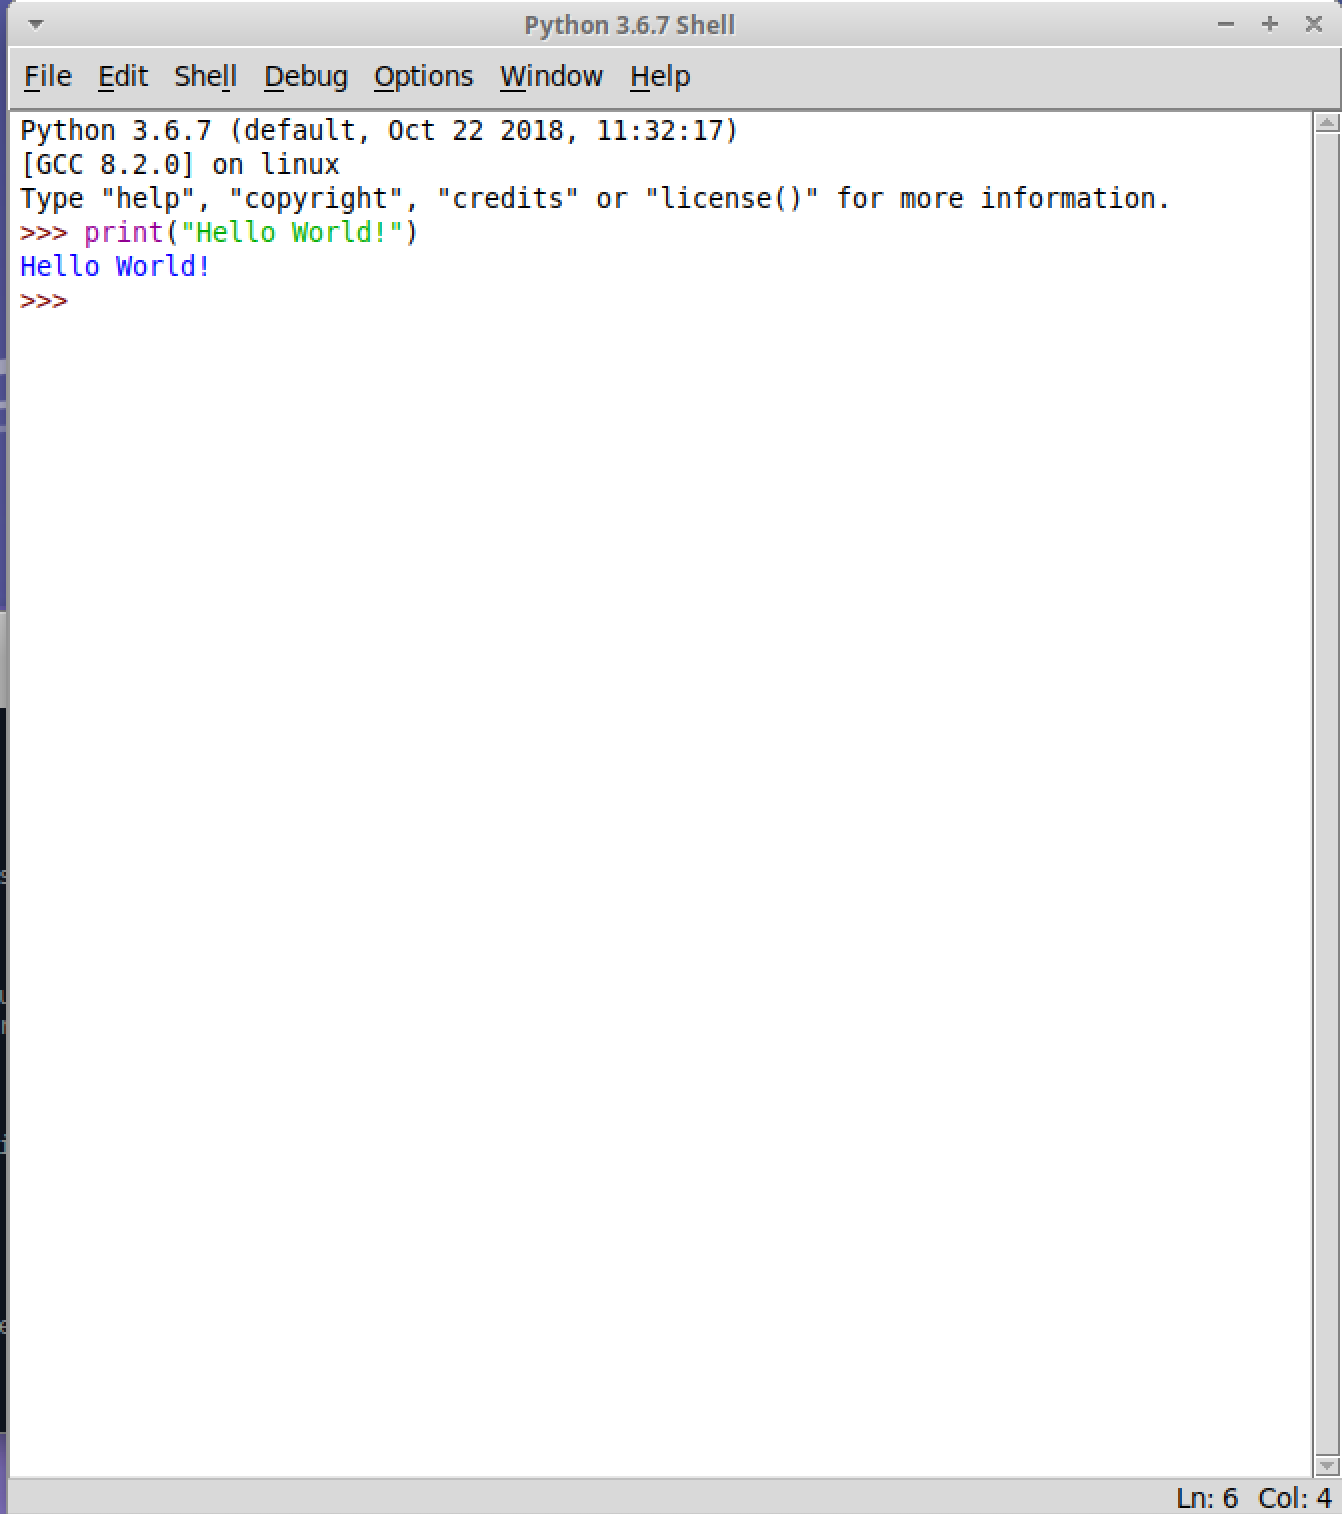
\includegraphics[scale=0.6]{screenshots/idlelinux-hw.png}
\end{myfigure}

In class today, you will start up IDLE for the first time, and type some commands in.

\section{Starting to Program in Python}

As you've read in Chapter 1 of the textbook, most computer programs perform three basic kinds of instructions:

\bi
    \item Input
    \item Processing
    \item Output
\ei

Your instructor will guide you through some examples of each in class.
% !TEX root = CSC104LectureNotes.tex

% \setcounter{chapter}{11}
\chapter{Python Errors and zyLabs}

\topquote{Syntax, my lad. It has been restored to the highest place in the republic.}{John Steinbeck}

\minitoc

\section{Python Errors}
\label{sec:errors}

If you are an athlete, or a performer, or a writer, or a pursuer of any other creative enterprise, you already know that part of the exhiliration of performing is the danger that something won't go the way you expect.  Programming a computer is no different.  Finding an error in a computer program is a common occurrence.  It has been nearly seventy years since a Major League Baseball player has successfully gotten a hit more than 40\% of the time in one season.  Baseball players don't look at outs as failures; they view them as opportunities to learn and improve.  You must be prepared to do the same if you are going to be a successful programmer.

\subsection{Syntax Errors}

\begin{myfigure}[float,label=fig:syntax-error]{Syntax Error: Calling a Function Without Parentheses}
    \centering
    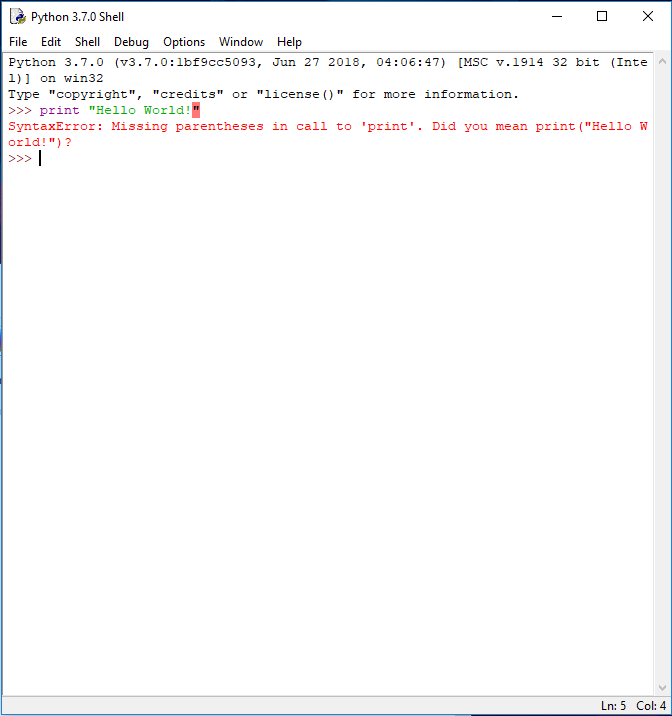
\includegraphics[scale=0.825]{screenshots/syntax-error}
\end{myfigure}

As you learned in Section 1.4 of zyBooks, and as we discussed way back on Day \ref{day:vocabulary} (see Section \ref{sec:kindsoferrors} in these notes), there are a couple of different kinds of errors we programmers can make.  The first kind of error is a \addindex{Error!Syntax error}{syntax error}.  As we learned then, a syntax error comes from writing an instruction that does not conform to the language's rules.

Yesterday, you wrote code that looks like this:

\begin{minted}{python}
print("Hello World!")
\end{minted}

As you now understand, that code is a \textit{call} to the \texttt{print} \textit{function}.  A \textbf{function call} such as this requires the use of parentheses.  If you tried to type this command without the parentheses, you would break the rules of Python's structure, and you would be informed of this immediately, as you see in Figure \ref{fig:syntax-error} on Page \pageref{fig:syntax-error}.

Notice that Python lets you know fairly clearly in red text that your error is a syntax error.  Sometimes (but not always), Python will also include a helpful hint regarding how you can fix this error, as it has in this example.

As you learn about more of Python's features, be sure to pay attention to the syntax that is required to make use of these features.  Like any programming language, Python can be very particular about how we type our code.

\subsection{Runtime Errors}

A \addindex{Error!Runtime error}{runtime error} is caused by a situation that the computer didn't expect.  Since a runtime error occurs when a program runs, such an error can only occur in code that is free of syntax errors.  Runtime errors typically cause the program to immediately terminate.

Consider this Python code that we looked at at the end of Day \ref{day:python1}:

\begin{minted}{python}
my_number = int(input('Type in a number: '))
print(my_number * 3)
\end{minted}

That Python program is free of syntax errors, and will run just fine as long as the user interacts with it in an expected way.  However, if you run the program and type \texttt{Idaho} instead of a number, the \mintinline{python}{int()} function won't be able to complete its job.  Python will respond with this error message:

\begin{tcolorbox}
\ttfamily\small ValueError: invalid literal for int() with base 10: 'Idaho'
\end{tcolorbox}

There are many kinds of runtime errors in Python, and you will not be required to know what they are.  As we write more code, however, you will encounter more errors and of more types, and you will gain experience in finding and fixing them.

\subsection{Semantic Errors}

A \addindex{Error!Semantic error}{semantic error}, or \textit{logic error}, is an error in a program's meaning.  Like runtime errors, these errors only occur in a program that can run (although a good programmer can detect them ahead of time).

Consider this program:
\begin{minted}{python}
age = int(input('How old are you?'))
months = age / 12
print("That's", months, "months!")
\end{minted}

That program will run to copmpletion and provide nice-looking output, which happens to be wrong.  The syntax is fine -- if it weren't, the program would not have run.  There were no runtime errors; the program provided its output and exited normally, with no red error messages.  The problem here is that the programmer provided the wrong instructions.  These kinds of errors are frequently referred to as \textit{bugs}.

\section{zyLabs}

Your instructor will have assigned several interactive programming assignments, to be completed during today's class.  These assignments are called \textbf{zyLabs}, and they're part of the zyBooks online textbook you signed up for.  It is important that you read the instructions for each assignment carefully before starting, and follow them as precisely as you can, to maximize your grade -- and to gain valuable hands-on experience programming in Python!  Remember to have fun, and to ask your instructor for help as soon as you think you need to.  There is no shame in asking for help, especially when trying to do something you have never done before.
% !TEX root = CSC104LectureNotes.tex

% \setcounter{chapter}{11}
\chapter{Variables and Expressions}

\topquote{Without memory, there is no culture. Without memory, there would be no civilization, no society, no future.}{Elie Wiesel}

\minitoc

\section{Variables}

As we started to explore on Day \ref{day:python1}, a \addindex{Variable}{variable} lets us store some information that we can use later.  Specifically, when we create a variable, we ask the computer to use a part of its \addindex{Memory}{memory}, or RAM, which we identify by name.  Later uses of that name keep referring to the same place in memory, so that we can retrieve what we stored.

\subsection{Assignment}

We create a variable by assigning a value to it, like you did when you typed \mintinline{python}{name = 'Olivia'}.  That equals sign in the middle has a special meaning to the Python interpreter.  It's called the \textbf{assignment operator}, and its presence in that statement makes it an \textbf{assignment statement}.  We use assignment statements to create variables, and to change their values.

\subsection{A Variable Has One Value}

If, later in the program, we type \mintinline{python}{name = 'Henry'}, then the name Olivia is removed from memory, and the name Henry takes its place in the variable called \texttt{name}.  If you need to store two pieces of information at the same time, you will have to make two variables, each with its own name.

\subsection{Identifiers}

Each variable must have a valid \addindex{Identifier}{identifier} -- that's a fancy word for ``name.''  Chapter 2 of the textbook discusses what identifiers are legal according to Python syntax, and what makes other Python programmers think an identifier is good.

\section{Objects}

In Python, variables are considered to be \addindex{Object}{objects}, and each object has a value, a type, and an identity.  The value is the data the object contains.  The type of an object is the same as the type of its value.  It's important to know that different data types sometimes disallow certain interactions -- for instance, you can't add 5 to ``Olivia''.

An object's identity allows us to tell whether two identifiers refer to the same object or not.  This is not important now, but it will be later.  What is important now is to see that an object's \textit{identifier} is its name, and its \textit{identity} is a reflection of how it is stored in memory.

We can use the Python function \mintinline{python}{type()} to get an object's type, and we can use the Python function \mintinline{python}{id()} to get an object's identity.

\section{Two Kinds of Numbers}

Programming languages differentiate between two different kinds of numbers.  An \addindex{Number!Integer}{integer} is a number that has no fractional or decimal component.  Programmers call numbers with decimal points \addindex{Number!Floating point}{floating-point numbers}, because of how they're stored in memory.  You will frequently hear programmers use the shortcuts \texttt{int} and \texttt{float} to refer to these data types, based on type names used in programming languages.

Just as there's an \mintinline{python}{int()} function to turn a string into an integer, there's a \mintinline{python}{float()} function to turn a string into a float.

In the next sections, you will learn to be careful when mixing numeric types in arithmetic expresssions.

\section{Expressions}

You can build up all sorts of mathematical expressions using variable names, literal values (like \texttt{5}), and operators.  Notice that some operators are \textit{unary}, like the negation operator in \texttt{-5}, while most operators are \textit{binary}, like the subtraction operator in \texttt{x - 5}.

It is considered good programming practice to leave a space around mathematical operators, because this makes code easier to read.  Consider:

\begin{minted}{python}
# An expresssion with no whitespace
x=31*y-14*(z-2)/17

# The same expression with a space surrounding each operator
x = 31 * y - 14 * (z - 2) / 17

# Which one would you rather read?
\end{minted}

Be sure to pay attention to the precedence rules when constructing an expression, because Python will always follow them when evaluating an expression.
% !TEX root = CSC104LectureNotes.tex

\chapter{Modules}
\label{day:modules}

\topquote{A computer is like a violin.  You can imagine a novice trying first a phonograph and then a violin. The latter, he says, sounds terrible.  That is the argument we have heard from our humanists and most of our computer scientists.  Computer programs are good, they say, for particular purposes, but they aren’t flexible.  Neither is a violin, or a typewriter, until you learn how to use it.}{Marvin Minsky}

\minitoc

\section{Where Your Files Go When You Save Them}

\subsection{The Department's Computers}

When you log in to the Windows computers in the Department of Mathematics, Computer Science, and Information Technology's labs in B Cluster, these computers make a couple of interesting resources available to you.  Of the most interest right now is a hard drive that is connected over the Department's network and mapped to drive \texttt{J:\textbackslash} (or ``the J drive'').  Because this is a network-mapped drive, you will always attach to the same J drive when you log in to any one of the computers in our computerized classrooms, or the Computer Learning Center in B 225, or even an instructor's computer in his or her faculty office.

For this reason, it is \textbf{\textit{strongly suggested}} that you save all files you create on one of the Department's computers to the J drive -- this way, there's less to remember.

It is important to know that any file you save to the C drive (the locally-mounted hard drive) on the Department's Windows computers is \textit{very likely to not exist} when you go looking for it.

\subsection{Your Computer}

Do you use your own computer during class?  Do you, or will you, use your own computer at home?  If so, you may already have an organization system set up, and you don't have to think much about where your new Python programs are going to be saved.  If not, then your computer is likely to suggest a suitable location.

In any case, make sure you know where your computer is storing files.  If you aren't sure of the location, it will be incredibly difficult for someone else to help you find these files later.

\section{Three Kinds of Python Programs}

As you can see in Section 2.8 of zyBooks, there are three basic ways of using IDLE to create Python programs.  So far, we have only been using the first, called \textit{interactive mode}.  Today, you will learn how to create \addindex{Script}{scripts} and \addindex{Module}{modules}.  Be sure to read Sections 2.8 and 2.9 carefully before class, pay attention during lecture, and ask any questions you have to as soon as they come up.  The work you do today will help you to understand these concepts, and create the tools you have to create when necessary.
% !TEX root = CSC104LectureNotes.tex

% \setcounter{chapter}{14}
\chapter{Strings and Numeric Types, and Writing a First Python Script}
\label{day:firstscript}

\topquote{I'm not a great programmer; I'm just a good programmer with great habits.}{Kent Beck}

\minitoc

\section{Strings}

You will learn after reading Chapter 3 of the zyBooks textbook that a string is a sequence of characters, and that we can do some interesting processing with the string as a whole, and its individual components as well.  After reading the chapter and completing the Participation Activities, you will be able to find the length of a string, compose a big string out of smaller strings, and determine which characters are in which places in a string.

\section{Numeric Types}

There are two types of real numbers in Python, \mintinline{python}{float} and \mintinline{python}{int}, which store different kinds of data and support different kinds of processing.  Understanding the similarities and differences will help you not just with today's work, but with many of the tasks you will have to complete this semester.

\section{Writing a Python Script}

In today's class, you will be given a new kind of homework assignment.  You will be tasked with writing a Python script and submitting it for grading.  This assignment is not a zyLabs assignment, and you won't receive automated feedback like you do from zyLabs.  Instead, you will write and test this script in IDLE, make sure for yourself that it works, and then submit it to your instructor for grading.  As the semester goes on, you will have more and more assignments like this.

It is, of course, of critical importance that the script you submit performs the right task.  However, we programmers demand more of ourselves than that.  Program code must also be easily read by humans.  As much as our source code conveys information to the computer, it must also convey information to us.  Therefore, it's a good idea to agree upon a standard way for our code to be formatted, so that we can see this information easily.

\section{The Header}
\label{sec:header}

While there is general consensus among the Python community, and the programming community generally, about what information should appear at the top of a source code file, there does not appear to be one standard regarding \textit{how} this information should be presented.  Presented here is the standard we will use, based upon commonly-used ideas and guidelines.

\subsection{The Shebang}
\label{sec:shebang}

The idea of ``scripting'', or ``writing scripts'', has been around longer than Python has, and in fact has been around longer than Microsoft Windows has.  Among the earliest kind of scripts are what are now referred to as ``shell scripts'', because they are sets of instructions for the \addindex{Command shell}{command shell}, or the interactive program that waits for the computer's user to type in commands.  In the earliest days of the Unix operating system, before graphical user interfaces, all of the instructions to the computer had to be typed at the shell.\footnote{The command shell in Unix is very powerful, and many programmers continue to choose to work with it rather than clicking things.}

\index{"\#"!@\texttt{"\#"!}} Unix users started writing scripts as a way to automate the stuff they had to type repeatedly to accomplish tasks.  These scripts need to start with a \addindex{Shebang}{shebang} to signal to Unix how to process the script.  The shebang consists of a ``sharp'' symbol (think music notation -- it's the \texttt{\#}) followed by a ``bang'' symbol, a programmer's shorthand for the \texttt{!} symbol.  A sharp and a bang together came to be known as a shebang.\footnote{Unix users have all sorts of fun names for things.  See Eric Raymond's Jargon File at \url{http://catb.org/jargon/html/}.}

A typical ``shell script'', therefore, would have a first line something like this:

\begin{verbatim}
#! /usr/bin/sh
\end{verbatim}

This tells Unix to use the program \texttt{sh}, located in the \texttt{/usr/bin} directory, to process the script.  Since we're working in Python, our shebang should look more like this:

\begin{verbatim}
#! /usr/bin/env python3
\end{verbatim}

This tells your Unix system to use the \texttt{env} program to figure out where Python 3 is installed, and use it to process the script.

You might be wondering at this point, if the shebang is a Unix thing, what effect it has on a Python script running on Microsoft Windows.  The developers of Python knew that people would want to run Python scripts on Windows, and so configured Python on Windows to safely ignore this line.  Therefore, you should provide a shebang at the top of every Python script.

\subsection{The Docstring}
\label{section:docstring}

Every Python script and module -- and certain program components that we will explore later -- should contain a \addindex{Docstring}{docstring} that provides a description of the code that follows.

While it is possible to fit a docstring on a single line, this is not the accepted standard for a script or a module.  We should include a multi-line docstring instead.

A docstring is really just a string, except that it starts and ends with \textit{three quote symbols} instead of one, like this:

\begin{minted}{python}
'''This is a docstring.

This is part of the same docstring.
'''
\end{minted}

While the Python specification \href{https://www.python.org/dev/peps/pep-0257/#multi-line-docstrings}{PEP 257} provides the most rigorous description of what to include in a docstring at the top of a script, we shall summarize it here:  The first line should contain a brief summary of the code, and then, following a blank line, the rest should consist of a more elaborate description.  If the script or module you're creating is part of an assignment, include the due date in the description.  The top of the Hello World script might, therefore, contain this after the shebang:

\begin{minted}{python}
'''Display a friendly message.

Display a friendly "Hello World" message to the user,
confirming that the computer's Python installation is in good
working order.

This script is part of Homework #1, due 2019-09-09.
'''
\end{minted}

\subsection{The Rest of the Header}

We shall define three special variables after the docstring (although in production code there are generally many more than these).  Assign the variable \mintinline{python}{__author__} a string containing your name, assign \mintinline{python}{__section__} a string containing the section of the class you're enrolled in, and assign \mintinline{python}{__email__} a string containing your email address.

% A complete Hello World script should, therefore, look like Code Listing \ref{lst:hwheader} on Page \pageref{lst:hwheader}.

\pyfile{Hello World With a Full Header}{hello-with-author-email.py}{hwheader}

% !TEX root = CSC104LectureNotes.tex

% \setcounter{chapter}{15}
\chapter{Python Conditionals}

\topquote{Truth can only be found in one place: the code.}{Robert C. Martin}

\minitoc

\section{Review: Conditional Statements}

If you've already forgotten everything you learned last month about conditional statements, it is probably best for you to go back to Day \ref{day:conditionals1} and re-read those sections.

\section{Python Conditionals}
\label{sec:pythonconditionals}

The material from earlier this semester will have you well-prepared to handle writing if statements in Python.  You already know how to identify the possible values and outcomes of a condition, and you largely already know how to write an if statement in Python.  As you read through Chapter 3 in zyBooks, there is very little new information to be gleaned.  Most importantly, pay attention to these items:

\subsection{Write Real Statements}
Where we previously wrote \textit{pseudocode} like this:

\begin{verbatim}
if major = CS:
    "You're a CS major"
elif major = IT:
    "You're an IT major"
else:
    "Your major is something else"
\end{verbatim}

The idea is there, but there are portions in that example that are not proper Python and won't compile.

\subsubsection{Relational Operators}

Recall that in Python, the \texttt{=} operator is used only for assignment.  When comparing two values in Python, we must use the \mintinline{python}{==} operator.

\subsubsection{String Literals}

When determining whether a variable like \mintinline{python}{major} contains a value like ``CS'', that value must either be stored in a variable already, or surrounded by double quotes.

\subsubsection{Displaying Output}

Before the first exam, it was enough to just write ``You're a CS major''.  Now, however, you've learned how to make a Python program display a string, so make sure to get that right.

\subsection{Indentation}

You will read about indentation in Chapter 3, but the important detail here is that you \textbf{\textit{must be consistent}} in how you use indentation.  Every statement at the same logical level must start in the same column of code.  For this reason, most Python programmers recommend that you indent four spaces at a time.

Therefore, the previous example should look like this in Python:

\begin{minted}{python}
if major == "CS":
    print("You're a CS major")
elif major == "IT":
    print("You're an IT major")
else:
    print("Your major is something else")
\end{minted}
% !TEX root = CSC104LectureNotes.tex

\chapter{The Software Development Life Cycle}
\label{day:bagels}

\topquote{Progress is possible only if we train ourselves to think about programs without thinking of them as pieces of executable code.}{Edsger W.\ Dijkstra}

\section{The Software Development Life Cycle}

The task of programming starts away from the computer.  Programmers don't just sit at a computer and start writing code that works; it takes careful planning and consideration to create a program that not only performs the job the programmer intended, but also addresses the need that first caused the programmer to start planning and writing.

Many thoughtful writers have tried to explain the steps involved in successful software creation, and so there is no one standard way to express what we do and how we do it.  But most expressions of the \addindex{Software Development Life Cycle}{software development life cycle} center around these six stages:

\begin{enumerate}
    \item \textbf{Understand the problem and the intended outcome.}  More than one programmer has developed a wonderful program for a client that doesn't do any of what the client asked for.
    \item \textbf{Design the solution.}  Once you understand what has to be done, fit the specification into your mode of working.  In this case, take the project requirements and turn them into an outline of a Python program.
    \item \textbf{Write the program.}  Once you have an idea of what you're going to write, sit down and write it.
    \item \textbf{Test and debug the program.}  The likelihood that your program is going to work the way you want the first time is inversely proportional to how important the program is.  Make sure it works, and fix it when it doesn't.
    \item \textbf{Create documentation.}  We have to write headers and comments, and sometimes we have to write blog posts and wiki articles and product manuals.
    \item \textbf{Deploy and maintain the product.}  For many programmers, the job isn't done when the program is written.  Some of us are responsible for making sure a program continues to work for months or even years after it first went into production.
\end{enumerate}

Today in class you are going to have some opportunities to work through the software development life cycle as we create some programs from problem description all the way through to finished product.
% !TEX root = CSC104LectureNotes.tex

\chapter{More Practice with Conditional Programming}
\label{day:movie-ticket}

\topquote{A problem well-put is half solved.}{John Dewey}

\section{More Conditional Programming}

Today your instructor will help you work through some more problem solving that requires programming conditional statements.  Remember to work through the  software development life cycle, and remember to develop test cases before you start coding.
% !TEX root = CSC104LectureNotes.tex

\chapter{Exam 2 Review}

Your instructor will have prepared some materials for you to review in class today.  Make sure to ask questions!

{\let\clearpage\relax\chapter{Exam 2}}

Good luck!

% !TEX root = CSC104LectureNotes.tex

\chapter{Introduction to Loops}

\topquote{Hofstadter’s Law: It always takes longer than you expect, even when you take into account Hofstadter’s Law.}{Douglas Hofstadter}

\minitoc

Can you write a program in Python that says ``Hello World!'' three times?  Sure you can.  How about ten times?  One hundred times?  You \textit{can}, but would you want to?  What kinds of mnistakes could you introduce when trying to write such a program?

In Section \ref{sec:threekinds} of these notes, you learned that there are three fundamental kinds of computer statements: sequential statements, selection statements, and iteration statements.  It is now time to learn about the last of these.

\section{Iteration}

One of the first goals of computer designers, even going back to Sir Charles Babbage,\footnote{\url{https://www.computerhistory.org/babbage/charlesbabbage/}} was that they would make life simpler by doing the sort of tasks that we humans didn't want to do.  In Chapter 4 of zyBooks, you will learn how Python makes it easy for us to tell the computer to automate certain tasks.

\section{Syntax}

Take care to notice that the syntax of a \addindex{Statement!Loop}{loop statement} is similar to that of a conditional statement: there's a keyword, a condition, a colon, and then a bunch of indented lines.  See these examples:

\begin{py}{If Statements and While Statements}{if-and-while}
x = 1

if x < 5:
    print("Hello from the if statement!")
    x += 1

print("More stuff happens here.")

while x < 5:
    print("Hello from the while statement!")
    x += 1

print("More stuff happens here.")
\end{py}

There's a big difference between the \mintinline{py}{if} statement and the \mintinline{py}{while} statement, however.  The body of the \mintinline{py}{if} statement runs at most once, but the body of the \mintinline{py}{while} loop will keep repeating as long as the condition is true.

Before class, see if you can determine what the outcome of this program will be, and then type it in and run it to see if you were right.

%%%%%%%%%%%%%%%%%%%%%%%%%%%%%%%%%%%%%%%%%%%%%%%%%%%%%%%%%%%%%%%%%%%%%%%%%%%%%%

\appendix
\appendixpage
\addappheadtotoc
% % !TEX root = CSC104LectureNotes.tex

\chapter{Number Systems}

\begin{table}[h]
    \begin{tabular}{rr}
        Decimal & Binary\\
        \hline
        0 & 0\\
        1 & 1\\
        2 & 10\\
        3 & 11\\
        4 & 100\\
        5 & 101\\
        6 & 110\\
        7 & 111\\
        8 & 1000\\
        9 & 1001\\
        10 & 1010\\
        11 & 1011\\
        12 & 1100\\
        13 & 1101\\
        14 & 1110\\
        15 & 1111\\
        16 & 1~0000\\
        \hline
    \end{tabular}
\end{table}
% !TEX root = CSC104LectureNotes.tex

\chapter{IDLE}
\label{chapter:idle}

\addindex{IDLE}{IDLE} is a simple graphical development environment for the Python programming language.  It is available for Windows, MacOS, and Linux.

IDLE provides an \textit{interactive} programming environment, as discussed in Section 1.2 of the textbook.  It also provides a way for you to run programs that were prepared earlier and saved.

\section{Using IDLE}

\subsection{Windows}

I downloaded Python from the official Python website, \url{https://www.python.org/downloads/}, and this download included IDLE.  Make sure to download the most recent available version of Python.  After running the installation program, I was able to run IDLE by pressing the Windows button in the lower left corner of the screen and then searching for IDLE.  When you initially run the program, you should see a window like the one in Figure \ref{fig:idlewin} on Page \pageref{fig:idlewin}.

\begin{myfigure}[label=fig:idlewin]{IDLE Running on Windows 10}
    \centering
    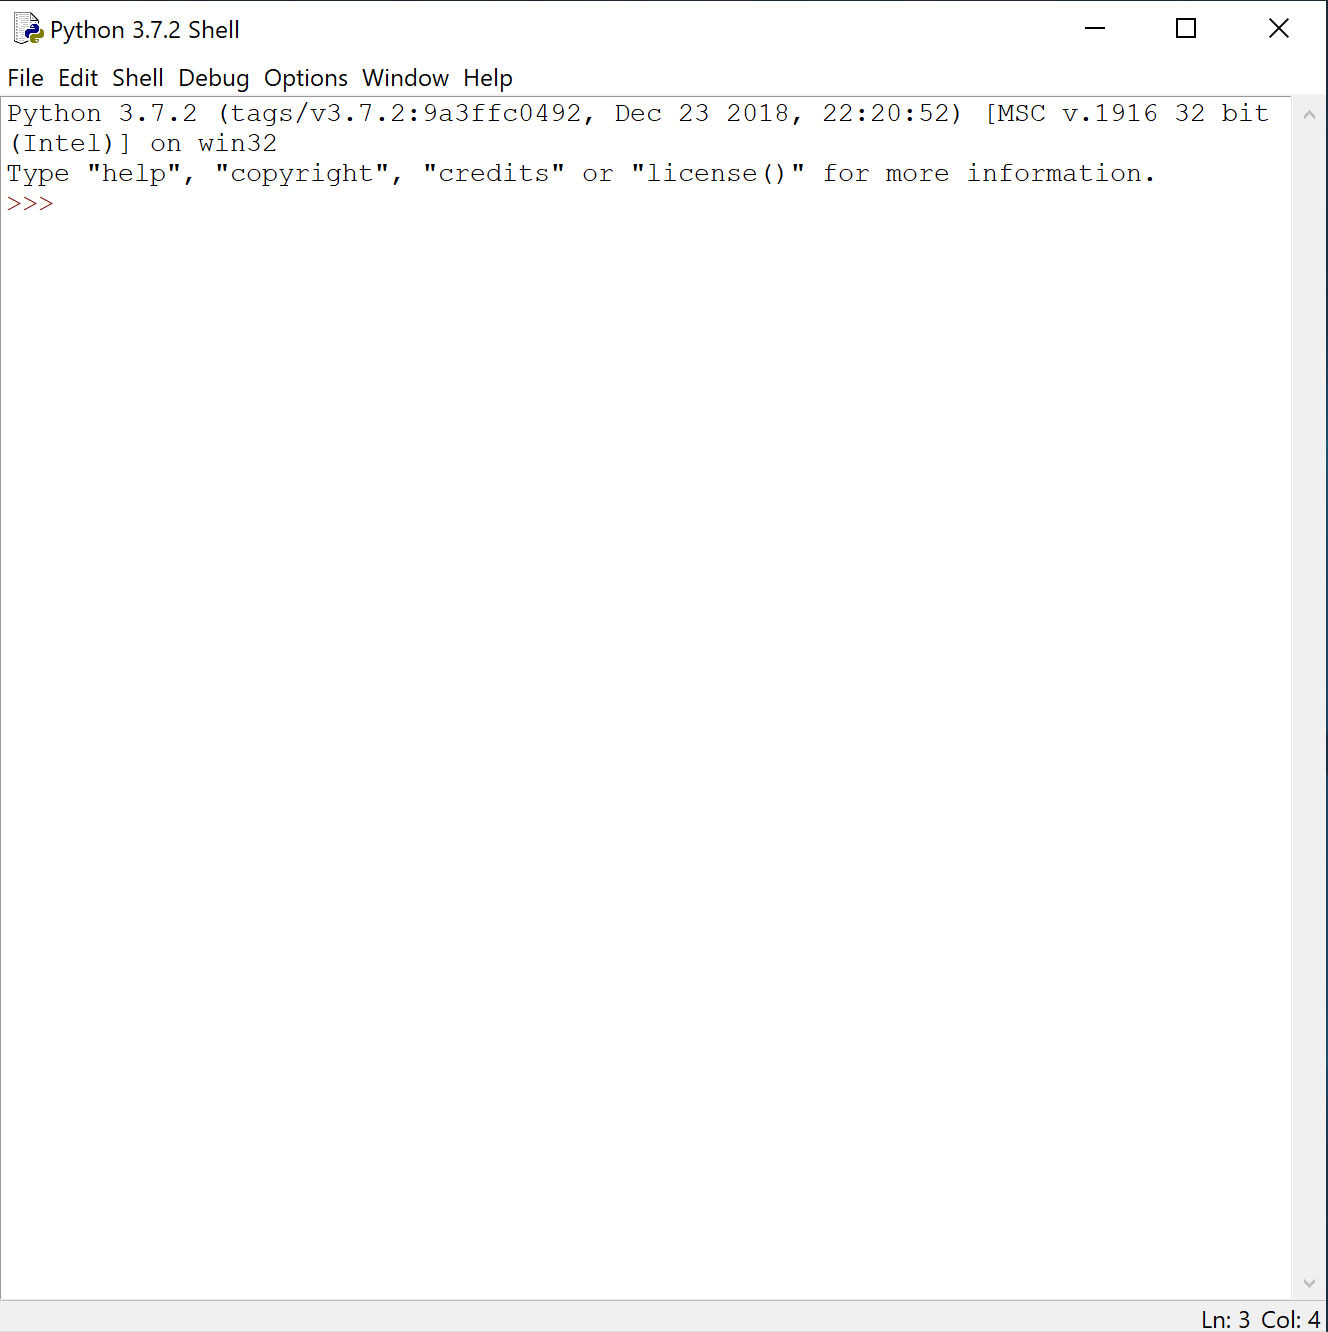
\includegraphics[scale=0.6]{screenshots/idlewin.png}
\end{myfigure}

Using the Option menu, I was able to change the font face to something nicer (I changed it to \href{Fira Code}{https://www.fontsquirrel.com/fonts/fira-code}, the same font used for code examples in these notes) and the font size to something more readable, as you see in Figure \ref{fig:idlewin-hw} on Page \pageref{fig:idlewin-hw}.

\begin{myfigure}[label=fig:idlewin-hw]{IDLE Running on Windows 10 with the Fira Code Font}
    \centering
    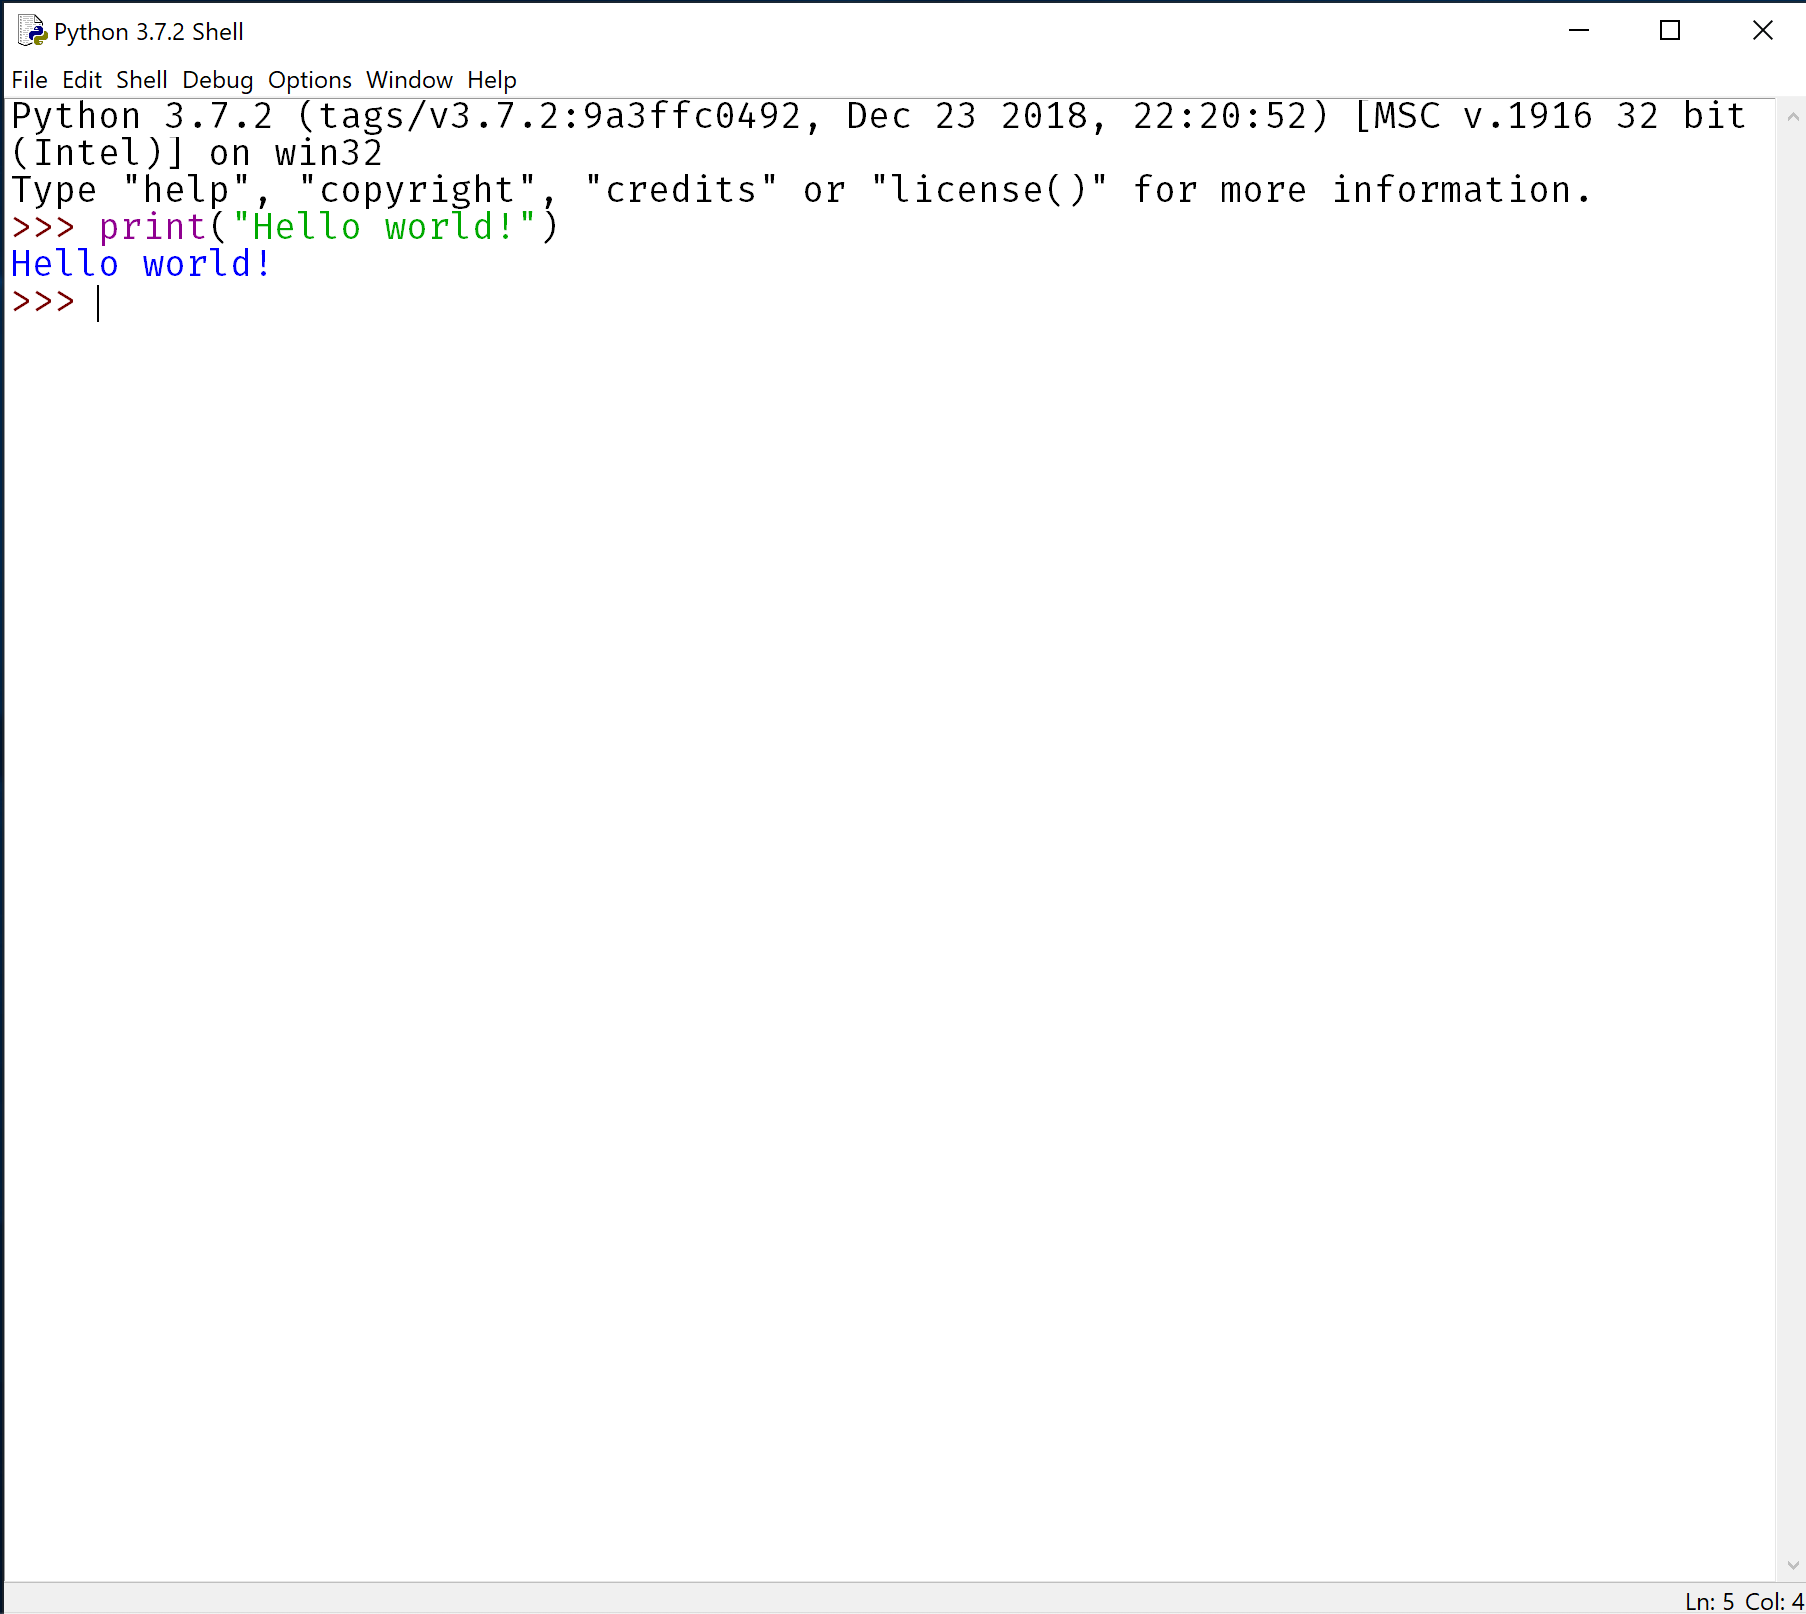
\includegraphics[scale=0.4]{screenshots/idlewin-hw}
\end{myfigure}

\subsection{Mac OS}

There are a couple of ways to install Python and IDLE for Mac OS, but the easiest way is probably the same as in Windows: to download the installation program from \url{https://www.python.org/downloads/} and install.

\subsection{Linux}

On my installation of Ubuntu Linux, I typed the following commands to install IDLE:

\begin{verbatim}
    $ sudo apt update
    $ sudo apt install idle
\end{verbatim}

You could also use the graphical software-installation tool to install IDLE.

Once it's installed, just type \verb-idle- at the command line prompt to open the program.  You should see something like the window in Figure \ref{fig:idlelinux} on Page \pageref{fig:idlelinux}.

\begin{myfigure}[label=fig:idlelinux]{IDLE Running on Ubuntu Linux}
    \centering
    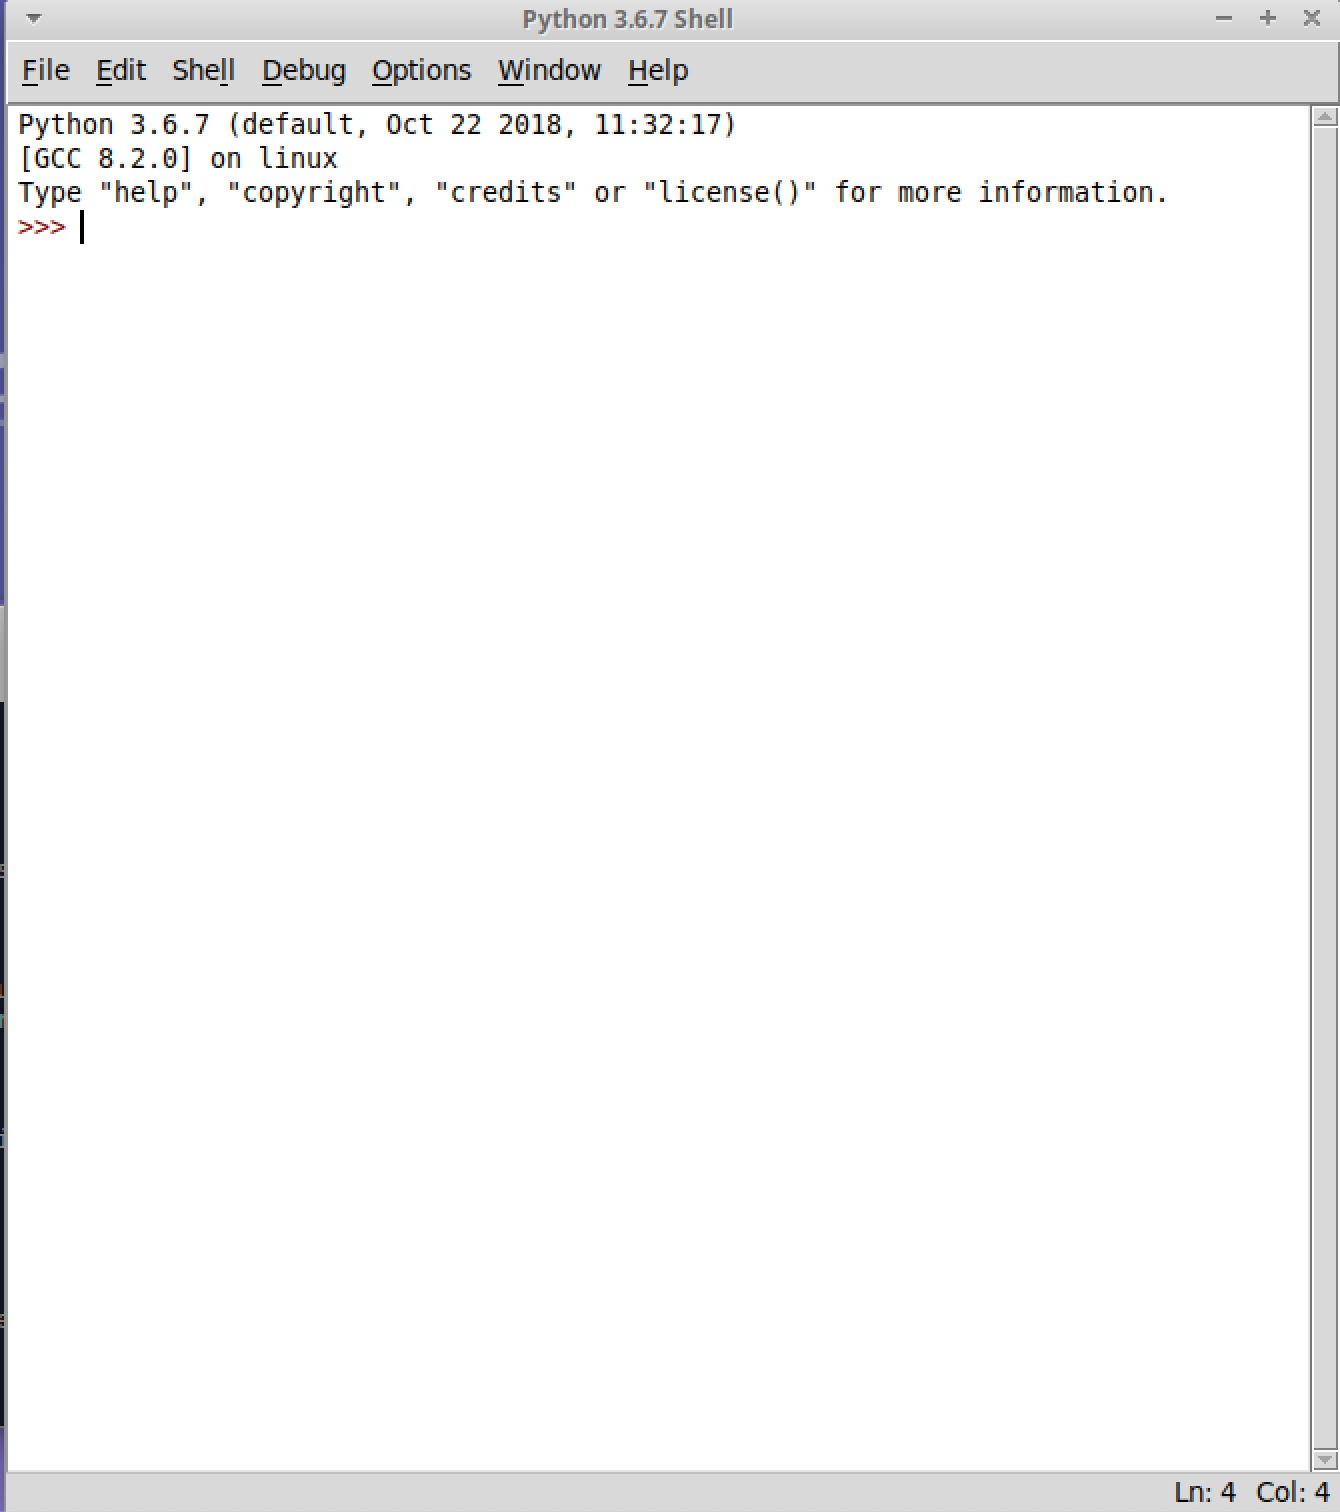
\includegraphics[scale=0.6]{screenshots/idlelinux.png}
\end{myfigure}

It is important that you see the phrase ``Python 3'' at the top of the screen (in this screenshot, it says ``Python 3.6.7'', and that's good).  If it says ``Python 2'' on the first line, then you are running an older version of IDLE -- and therefore an older version of Python -- and things won't work the way you expect.  If this is the case, try running \verb-idle3- instead of just \verb-idle-.  If that doesn't work, try to use \verb-apt- to install \verb-idle3-.
% !TEX root = CSC104LectureNotes.tex

\chapter{Python Keywords}

\index{Reserved words|see {Keywords}}\addindex{Keywords}{Keywords} are words that have a special meaning in Python.  As discussed in XXXXX, we are not allowed to use keywords as identifiers.

This table was copied from this list at W3Schools: \url{https://www.w3schools.com/python/python_ref_keywords.asp}.

Notice that all of these keywords consist completely of lowercase letters except for \texttt{False}, \texttt{True}, and \texttt{None}.

\bigskip

\newcolumntype{K}{%
    >{\raggedleft\ttfamily}p{0.2\textwidth}
}

\topcaption{The Keywords of the Python Language} \label{tab:keywords}

\tablefirsthead{\hline \multicolumn{1}{r}{\textbf{Keyword}} &
    \multicolumn{1}{l}{\textbf{Meaning}} \\ \hline }
    
\tablehead{\multicolumn{2}{c}%
    {{\captionsize\bfseries \tablename\ \thetable{} --
    continued from previous page}} \\
    \hline \multicolumn{1}{r}{\textbf{Keyword}} &
    \multicolumn{1}{l}{\textbf{Meaning}} \\ \hline }

\tabletail{\hline \multicolumn{2}{r}{{\textit{Continued on next page}}} \\}
\tablelasttail{\hline \hline}

\xentrystretch{-0.175}

\begin{xtabular}{K p{.80\textwidth}} 
    and & A logical operator\\
    as & To create an alias\\
    assert & For debugging\\
    break & To break out of a loop\\
    class & To define a class\\
    continue & To continue to the next iteration of a loop\\
    def & To define a function\\
    del & To delete an object\\
    elif & Used in conditional statements, same as else if\\
    else & Used in conditional statements\\
    except & Used with exceptions, what to do when an exception occurs\\
    False & Boolean value, result of comparison operations\\
    finally & Used with exceptions, a block of code that will be executed no matter if there is an exception or not\\
    for & To create a for loop\\
    from & To import specific parts of a module\\
    global & To declare a global variable\\
    if & To make a conditional statement\\
    import & To import a module\\
    in & To check if a value is present in a list, tuple, etc.\\
    is & To test if two variables are equal\\
    lambda & To create an anonymous function\\
    None & Represents a null value\\
    nonlocal & To declare a non-local variable\\
    not & A logical operator\\
    or & A logical operator\\
    pass & A null statement, a statement that will do nothing\\
    raise & To raise an exception\\
    return & To exit a function and return a value\\
    True & Boolean value, result of comparison operations\\
    try & To make a try...except statement\\
    while & To create a while loop\\
    with & Used to simplify exception handling\\
    yield & To end a function, returns a generator\\
\end{xtabular}


\backmatter

\addcontentsline{toc}{chapter}{Index}
\printindex
\end{document}
